\documentclass[12pt]{article}
\usepackage[labelfont=bf]{caption}
\usepackage{amssymb}
\usepackage{amsfonts}
\usepackage{amsmath}
\usepackage[nohead]{geometry}
\usepackage[singlespacing]{setspace}
\usepackage[bottom]{footmisc}
\usepackage{indentfirst}
\usepackage{endnotes}
\usepackage{graphicx}
\usepackage{rotating}
\usepackage{hyperref}
\usepackage{enumitem}

% due to Subfloats section in  
% http://en.wikibooks.org/wiki/LaTeX/Floats,_Figures_and_Captions
\usepackage{graphicx}
\usepackage{caption}
\usepackage{subcaption}

\usepackage{float}

\usepackage{array}
\usepackage{longtable}
\usepackage{fullpage}
\usepackage{dcolumn}
\usepackage[flushleft]{threeparttable}
\usepackage{booktabs}
\usepackage[12hr]{datetime}
\usepackage[DIV=16]{typearea}
\usepackage{scrextend,booktabs}
\usepackage{tabulary}
\usepackage{multirow}
\usepackage[font=footnotesize]{caption}

% due to 
% \usepackage{graphicx}
\usepackage{wrapfig}
\usepackage{lscape}
% \usepackage{rotating}
\usepackage{epstopdf}

\setcounter{MaxMatrixCols}{30}
\newtheorem{theorem}{Theorem}
\newtheorem{acknowledgement}{Acknowledgement}
\newtheorem{algorithm}[theorem]{Algorithm}
\newtheorem{axiom}[theorem]{Axiom}
\newtheorem{case}[theorem]{Case}
\newtheorem{claim}[theorem]{Claim}
\newtheorem{conclusion}[theorem]{Conclusion}
\newtheorem{condition}[theorem]{Condition}
\newtheorem{conjecture}[theorem]{Conjecture}
\newtheorem{corollary}[theorem]{Corollary}
\newtheorem{criterion}[theorem]{Criterion}
\newtheorem{definition}[theorem]{Definition}
\newtheorem{example}[theorem]{Example}
\newtheorem{exercise}[theorem]{Exercise}
\newtheorem{lemma}[theorem]{Lemma}
\newtheorem{notation}[theorem]{Notation}
\newtheorem{problem}[theorem]{Problem}
\newtheorem{proposition}{Proposition}
\newtheorem{remark}[theorem]{Remark}
\newtheorem{solution}[theorem]{Solution}
\newtheorem{summary}[theorem]{Summary}
\newenvironment{proof}[1][Proof]{\noindent\textbf{#1.} }{\ \rule{0.5em}{0.5em}}
\makeatletter
\def\@biblabel#1{\hspace*{-\labelsep}}
\makeatother
\geometry{left=1in,right=1in,top=1.00in,bottom=1.0in}
\setlength{\parskip}{1em} 

\begin{document}

\title{Unraveling a secret: Vietnam's outstanding performance on the PISA tests}
\author{Suhas D. Parandekar\thanks{e-mail for corresponding author: \textit{sparandekar@worldbank.org}  This paper has been written using open source software: R for the econometric analysis and graphics and LaTeX for typesetting. Thanks to all who make free software possible and to OECD for making the PISA data freely and easily available to anyone. The code used in writing this paper is freely available for download at \href{http://economist-at-work-and-play.blogspot.com/2015/02/pisa20121a.html}{http://economist-at-work-and-play.blogspot.com/2015/02/pisa20121a.html}}
\\Elisabeth K. Sedmik\medskip\\
{\normalsize Global Practice for Education, The World Bank} 
\date{\normalsize Date of this draft: \today }}
\maketitle

\sloppy

\singlespacing

\textbf{Abstract}

This paper presents an analyis of the factors that explain Vietnam's outstanding performance on the PISA assessment in 2012. The paper presents a comparative analytical perspective between Vietnam and Colombia, using an Oaxaca-Blinder decomposition of a test score production function. The findings reveal that a) b) and c). 

\strut

\textbf{Keywords:} PISA;Vietnam;Colombia;Oaxaca-Blinder Decomposition; Economics of Education.

\strut

\textbf{JEL Classification Numbers:} I21 (Analysis of Education); I28(Government Policy); Z18(Public Policy).

\thispagestyle{empty}

\pagebreak%
\onehalfspacing
%\doublespacing

\section{Introduction}
Vietnam participated in PISA for the first time in 2012 and its performance has been much higher than other developing countries that take part in this OECD led initiative. PISA scores are calibrated to an OECD mean of 500 and standard deviation of 100 points. Only a few developing countries take part in PISA, perhaps because most of them have results much lower than the OECD countries. As can be seen in Figure 1, there is a positive, albeit non-linear correlation between GDP per capita and PISA test scores that can be seen by the dashed line representing a loess regression. The figure shows that Vietnam's performance in PISA (mathematics mean score of 511) is closer to that of Finland and Switzerland rather than of Peru and Colombia. Vietnam, represented by a red star in Figure 1, lies much above the cluster of developing countries in the lower left hand corner of Figure 1.  

\begin{figure}[H]
   \caption{\textbf{PISA 2012 results compared with GDP per capita}}
   \centering 
     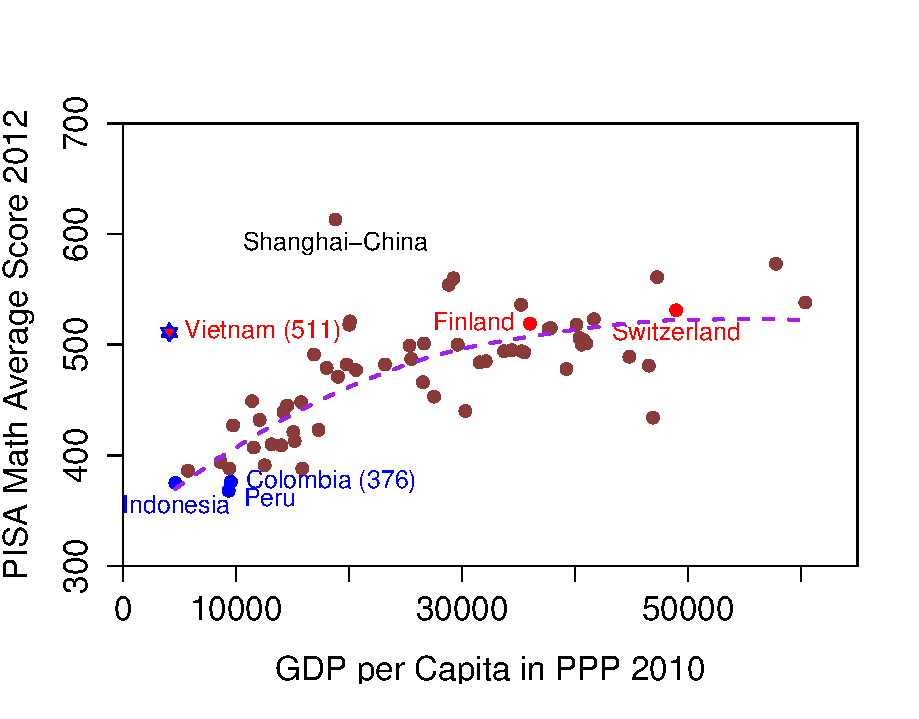
\includegraphics[width=0.75 \textwidth]{INTRFIG1.pdf} \\
\scriptsize{Source:OECD-PISA database        \hspace{3in}     }
   \label{Figure 1} 
\end{figure}

In the OECD-PISA database, there are seven countries other than Vietnam with a per capita GDP (in PPP dollars) below US\$ 10,000 - Albania, Colombia, Indonesia, Jordan, Peru, Thailand and Tunisia.  Their collective weighted average performance in mathematics was a mean score of 383. It is helpful to understand the significance of the 128 point difference with Vietnam. According to a recent OECD publication (\cite{OECD2013a}) \emph{``An entire proficiency level in mathematics spans about 70 score points \textendash  
a large difference in the skills and
knowledge students at that level possess. Such a gap represents the equivalent of about two years of schooling in the typical OECD country.''} Applying this heuristic would imply a nearly 3 year difference in attainment between Vietnam and the group of 7 developing countries in the PISA database. It should be noted at the outset that cross-section data from one instalment of PISA does not permit causal inference, but correlations can still provide useful insights. The difference is not only for mathematics and not just in the mean score, but spanning the entire test distribution, as can be seen in Figure 2.

\begin{figure}[H]
\caption{\textbf{Kernel Density comparison between Vietnam and other Developing Countries}}\label{fig:Kernel}
         \centering
         \begin{subfigure}[b]{0.3\textwidth}
                 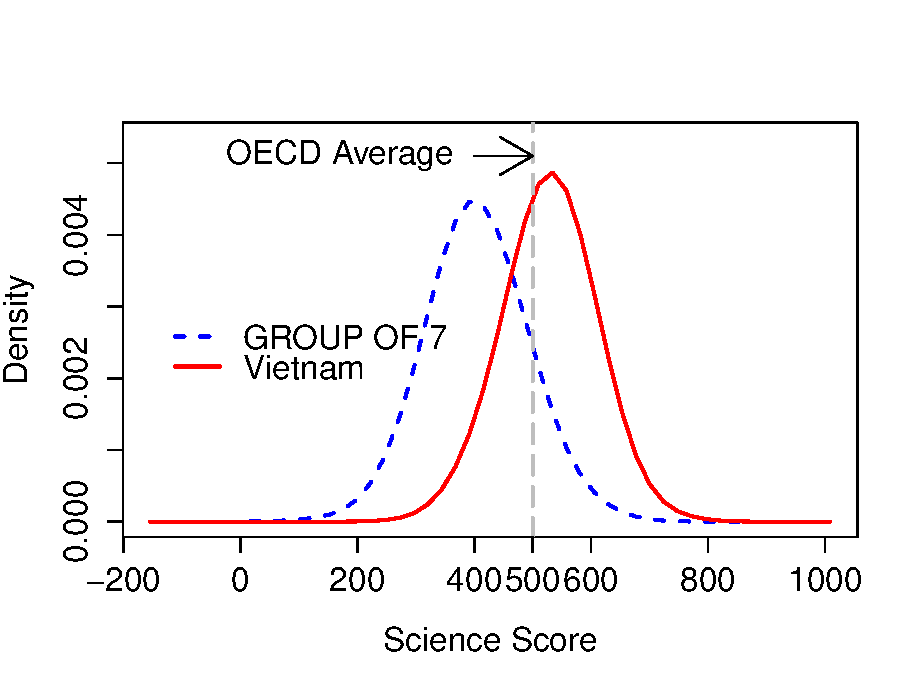
\includegraphics[width=\textwidth]{INTRFIG2a.pdf}
                 \caption{Science}
                 \label{fig:science}
         \end{subfigure}%
         ~ %add desired spacing between images, e. g. ~, \quad, \qquad, \hfill etc.
           %(or a blank line to force the subfigure onto a new line)
         \begin{subfigure}[b]{0.3\textwidth}
                 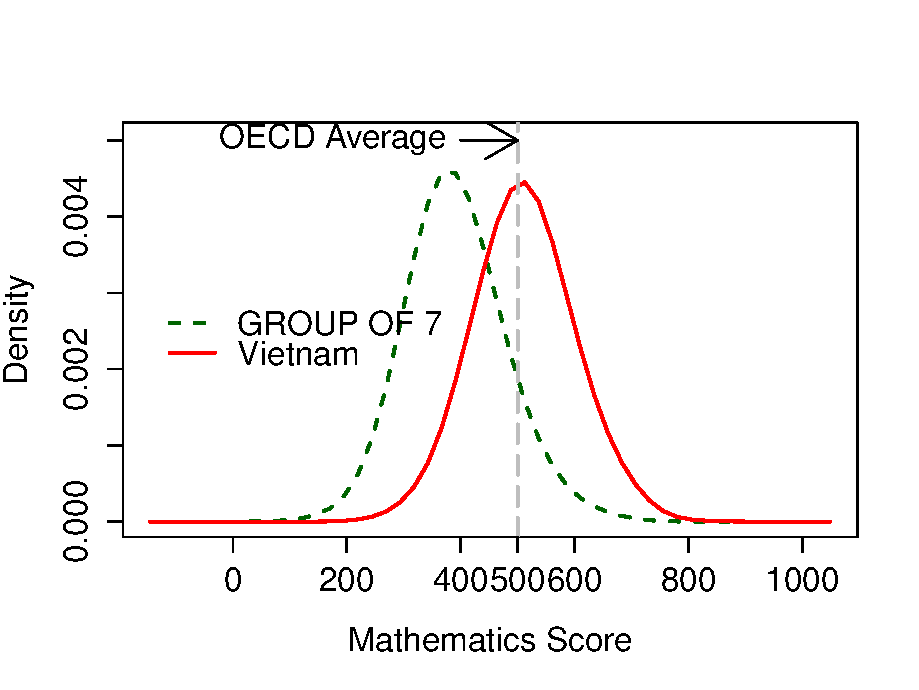
\includegraphics[width=\textwidth]{INTRFIG2b.pdf}
                 \caption{Mathematics}
                 \label{fig:mathematics}
         \end{subfigure}
         ~ %add desired spacing between images, e. g. ~, \quad, \qquad, \hfill etc.
           %(or a blank line to force the subfigure onto a new line)
         \begin{subfigure}[b]{0.28\textwidth}
                 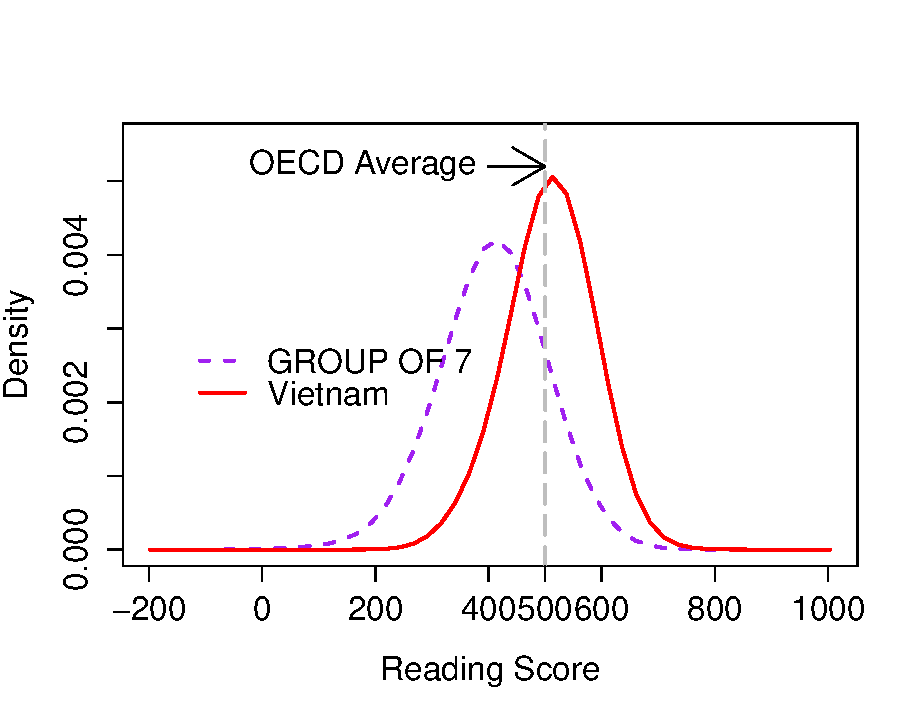
\includegraphics[width=\textwidth]{INTRFIG2c.pdf}
                 \caption{Reading}
                 \label{fig:reading}
         \end{subfigure}
     \end{figure}

A range of alternative classifications are possible to organize the possible explanatory factors available in the OECD-PISA database. Figure 3 presents four sets of factors, starting clockwise from the right. This is admittedly an arbitrary classification, utilized merely for expository purposes as we consider each of the constituent variables in turn. 

\begin{figure}[H]
   \caption{\textbf{Conceptual Scheme based on available comparative variables}}
   \centering 
     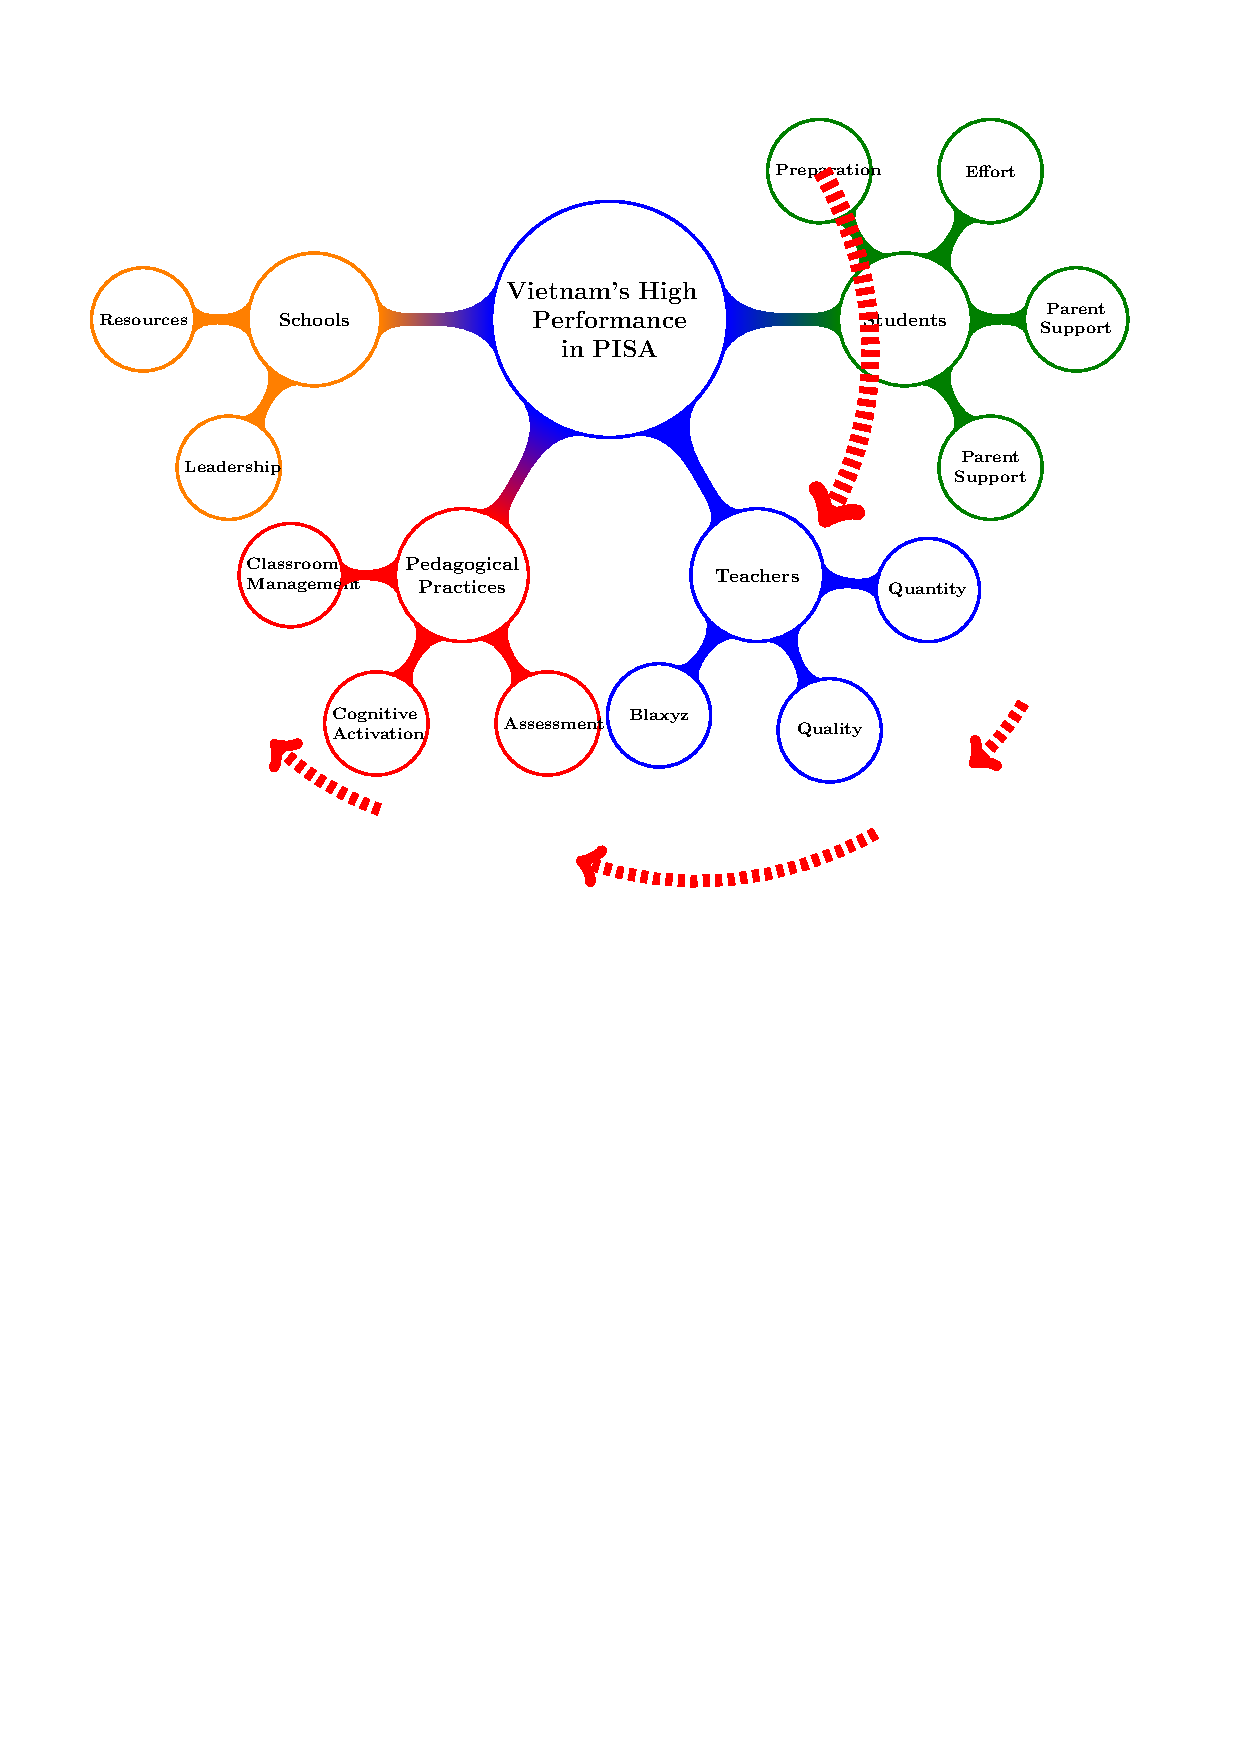
\includegraphics[width= 5in]{INTRTIKZ.pdf} \\
   \label{fig:m} 
\end{figure}

The approach of this paper is as follows. We begin in Section 2 by examining closely the differences in endowments between Vietnam and the collective group of 7 developing countries, termed as Dev7 for this paper (not to be confused with the G-7 of wealthy countries). The word `endowments' is used in a general sense, referring not merely to wealth related variables such as school resources, but to the range of policy, attitudinal and reported practices in the PISA dataset. The variables can also be considered as exogenous variables for the purpose of this analysis - in the first section we examine the mean differences in the levels of these variables. Comparing means in this context is a first pass at understanding the performance anomaly of Vietnam on empirical grounds. Without any priors, we want to look at seemingly obvious possible explanation - that Vietnamese 15 year olds somehow enjoy better endowments - economic, social, cultural and so on. This first pass can be quite revealing. For instance, even though we know that Vietnam's GDP per capita is the lowest in this G8 group of countries, perhaps the Vietnamese government and people have invested heavily in basic education, and schools in Vietnam enjoy much higher quality of facilities and equipment. Or the teachers have much higher level of education, and so on. Alternatively, one could find empirically that the schools are worse equipped and the teachers poorly trained. An examination of mean differences will provide us with a first set of tentative hypotheses.
\par
We make a second closer approach in Section 3 by adopting the regression methodology used by Fryer and Levitt in understanding differences in test score results of black children in the United States \cite{FryerLevitt04}. Differences in mean values of endowments leave some questions unanswered, which further analytical approaches can seek to resolve. In a multi-variate setting, we can try to understand how much of the variation can be explained by differences in observable endowments, and how much can be attributed to effects other than the observable differences. Fryer and Levitt have quite successfully followed the approach to explain what they see as evidence of a systemic difference in schools attended by black children. We adopt a similar approach to find out how much of the 'Vietnam gap' could reasonably be attributed to the earlier differences in mean endowments. As a matter of fact, we show in this section that the large differences in mean endowments is important, but it explains at best only half of the test score differences. 

The Fryer and Levitt method deepens the understanding from mean comparisons, but what it does not reveal may be as interesting as what it does reveal. Our Fryer-Levitt adaption is based on a pooled regression of eight developing countries, where we follow the fate of the magnitude of the coefficient of the dummy variable representing the Vietnamese student in the sample.  But we also need to investigate structural differences in the effects of endowments between Vietnam and Dev7 countries. In Section 4, we adopt an approach first used to explain variation in PISA performance between Germany and Finland by Andreas Ammermueller \cite{Ammermueller07}. This is an adaptation of the popular Oaxaca-Blinder decomposition of wage earnings equation to uncover evidence of discrimination on the basis of gender. \cite{Blinder73} and \cite{Oaxaca73} In this section, we can examine closely the structural differences between Vietnam and the Dev7 countries, including the contribution of differences in endowments and the coefficients to the gap in test scores. 

Even a multi-variate regression approach only proves correlation with nothing more than a hint regarding causation, and so far we have only one year (2012) of PISA data for Vietnam. PISA 2015 data will be available in 2016 and analytical approaches closer to establishing causality can be attempted. Even with the caveat regarding causality, there are useful policy related conclusions that we can derive from the analysis presented in this paper - learning for Vietnam, with regard to areas of strengths and weaknesses; and learning for other countries that may wish to emulate aspects of Vietnam's performance. There is a veritable industry of papers regarding Finland's PISA performance, directed mostly towards other OECD countries with lower scores, for instance United States. Vietnam's superlative performance points to a similar future stream of research, with the added advantage of relevance for developing countries. Section 5 provides concluding ideas that might be amongst the first of many more such ideas from future investigations of Vietnam's performance. 


\section{Endowment Differences regarding Student, Family, Teachers and Schools}

\subsection{Student Characteristics and Background}

An examination of fixed students characteristics (gender and age) does not show any statistically significant differences (Table 1). The PRESCHOOL variable shows the first instance of a statistically siginificant difference. While 78.88\% of Dev7 students reported attending preschool, the number of students attending preschool from the Vietnam sample was 91.20\% - a sizeable difference both statistically and economically significant. The relationship between preschool and later outcomes has been studied very closely over the years. Longitudinal impact evaluation studies regarding the Perry preschool project and Head Start in the US are amongst the most cited studies in the economics literature\footnote{For detailed meta-analysis, see \cite{Barnett95} and \cite{Schweinhartetal05}}. Of course, mean differences for PRESCHOOL and other variables reported in this section can only indicate possible explanations to be explored further. We can also see from the numbers for REPEAT in Table 1 that PISA takers in Vietnam were three times less likely to have repeated a grade in the past (6.79\% compared to 19.15\%).

\begin{table}[H]
	\tiny
	\def\arraystretch{0.9}
	\centering
	\caption{\textbf{Student characteristics and family background}}
	\begin{tabulary}{1.0\textwidth}{L L C C C C}
		\hline\hline \\
		\multicolumn{2}{c}{}
		& \multicolumn{2}{c}{Dev7 countries}
		& \multicolumn{2}{c}{Vietnam}	\\
		\hline & & & & & & 
		Variable & Description & MS & Valid N &  MS & Valid N \\
		\hline \\
		\multicolumn{6}{l}{\textbf{Fixed characteristics}}	\\ [0.3em]
      \hline \\
		FEMALE & Sex of student & 0.5265 & 41394 & 0.5336 & 4882 \\ 
		& & (0.4993) &  & (0.4989) &  \\ [0.3em]
      AGE & Age of student & 15.xxxx & 41394 & 0.xxxx & 4882 \\ 
		& & (0.xxxx) &  & (0.xxxx) &  \\ [0.3em]
     \hline \\
     \multicolumn{6}{l}{\textbf{Student's prior history}}	\\ [0.3em]
     \hline \\ 
		PRESCHOOL & Attended Preschool & 0.7888 & 40114 & 0.912 & 4866 \\ 
		&  & (0.4082) &  & (0.2833) &  \\ 
		REPEAT & Grade repeating & 0.1915 & 40343 & 0.0679 & 4860 \\ 
		& &  (0.3935) &  & (0.2516) &  \\ [0.3em]
     \hline \\
     \multicolumn{6}{l}{\textbf{Truancy from School}}	\\ [0.3em]
     \hline \\ 
		ST08Q01 & Times late & 1.5131 & 40663 & 1.1872 & 4873 \\ 
		& for school & (0.7648) &  & (0.4685) &  \\ [0.3em]
		ST09Q01 & Days unexcused & 1.2192 & 40650 & 1.0999 & 4875 \\ 
		& absence & (0.5276) &  & (0.3527) &  \\ [0.3em]
		ST115Q01 & Times skipped & 1.2585 & 40632 & 1.0764 & 4880 \\ 
		& classes & (0.545) &  & (0.3216) &  \\ [0.3em]
     \hline \\
     \multicolumn{6}{l}{\textbf{Parental background and family wealth}}	\\ [0.3em]
     \hline \\ 
		HISEI & Highest parental & 40.4196 & 32814  & 26.6023 & 4860 \\ 
		& occupational status & (22.5168) &  & (19.855) &  \\ [0.3em]
		MISCED & Educational level & 3.1193 & 40486 & 2.1744 & 4844 \\ 
		& of mother (ISCED) & (1.9853) &  & (1.6059) &  \\ [0.3em]
		WEALTH & Family wealth & -1.4606 & 40821 & -2.1343 & 4881 \\ 
		& possessions & (1.2267) &  & (1.1656) &  \\ [0.3em]
		CULTPOS & Cultural possessions & -0.1424 & 39905 & -0.2361 & 4809 \\ 
		& & (0.9678) &  & (1.0173) &  \\ [0.3em]
		HEDRES & Home educational &  -0.7427 & 40579 & -1.0743 & 4874 \\ 
		& resources & (1.1473) &  & (0.9364) &  \\ [0.3em]
		BOOK\_N & Number of books & 53.6393 & 39631 & 50.786 & 4841 \\ 
		& in family home & (94.5556) &  & (75.4031) &  \\[0.3em]
		\hline \\
	\multicolumn{6}{l}{Notes: The variables relate to the questionnaires administered to students in the general}\\    
	\multicolumn{6}{l}{(non-rotated) booklet. For a more detailed description of variables, please see Table xx.}\\
	\multicolumn{6}{l}{Items marked with \textit{(r)} are taken from the rotated student questionnaire. The variable}\\
	\multicolumn{6}{l}{means of Dev7 and Vietnam are statistically different at the 95\% significance level, except}\\
	\multicolumn{6}{l}{FEMALE.}\\
\end{tabulary}
\end{table}
The finding regarding PRESCHOOL and REPEAT indicates the possible importance of the trajectory of the student prior to High School. Repetition rates are difficult as comparative indicators of system quality because of the variations across countries in curriculum and standards, but REPEAT is another interesting variable to keep in mind as a possible clue to the mystery of Vietnam's PISA performance. As in some other East Asian cultures, Vietnamese children are expected by their parents to study hard. Though Mark Twain in Vietnamese translation is quite a best seller for young readers in Vietnam, truancy from school is not perceived benovelently by parents.\footnote{A cultural explanation is possibly quite important in explaining Vietnam's anomalous PISA results, though the PISA dataset may only be able to measure the possible effects of culture rather than measuring cultural differences. Literature from the World Values Survey, that does seek to measure cultural differences, indicates that Vietnam is a positive outlier on discipline and authority orientation\cite{DaltonOng05}.} Table 1 indicates a consistently lower truancy rate for the three variables used - the question refers to the past week \textbf{(to confirm)} and Vietnamese students are less likely to be late for school, have fewer days of unexcused absence and skip fewer classes. 

The final set of variables in Table 1 concern parental background and wealth at the students home, including cultural resources and books at home which may work to stimulate cognitive development. The PISA database includes a number of indices to measure aspects such as weath and possessions. These indices are based on underlying data regarding occupations and possessions. The scaling of raw data to indices is described in detail in the PISA technical report \cite{OECD2014a}. For HISEI, the parents occupation status, the OECD mean is 50 and the OECD standard deviation is 15. Table 1 shows that the HISEI for Dev7 parents at 40.42 was much higher than 26.60 for Vietnamese parents. MISCED refers to the International Standard Classification of Education (ISCED) developed by UNESCO. Table 1 shows that the average level of mother's education for Dev7 was just over 3, meaning Upper Secondary education, while for Vietnam the mean was just over 2, meaning Lower Secondary education. The WEALTH index is set for an OECD mean of zero and standard deviation of 1. Dev 7 countries wealth level was -1.5 and Vietnam's was -2.1, consistent with the data regarding occupational classification and mother's education. These findings indicate the close correlation of these variables with GDP per capita. The more interesting finding concerns the indices CULTPOS and HEDRES, which have OECD mean 0 and s.d. 1, and the number of books. CULTPOS includes classical literature, books of poetry and works of art. HEDRES includes reference books and books to help with school work as well as a study desk and 'a quiet place to study'. These three variables are also in line with per capita income - with the Dev7 mean being lower than the OECD mean, and Vietname being lower than Dev7. So one explanation regarding Vietnam's PISA performance can probably be ruled out - it does not seem likely that Vietnamese households spend disproportionately higher amount of their incomes on acquiring possessions that would give their children an edge in life. Books and other education related articles are owned by Vietnamese households to the same extent as any other households. 

\subsection{Student studying time out of school}

The phenomenon of primary and high school children taking extra classes to supplement in school instruction in Vietnam is well known \cite{HaHapharm05} and \cite{Hai-Anh07}. Table 2 indicates that while Dev7 students spent roughly 4.7 hours in such classes (total of OUTMATH, OUTLANG and OUTSCIE), the Vietnamese student spent nearly 2 hours more for a total of 6.6 hours, with the difference being highest for OUTMATH. Vietnamese students also spent about 1 additional hour per week doing homework (total of ST57Q01 and ST57Q02) compared to Dev7 students. The highest difference in this set of variables concerns the variable ST57Q04, which relates to extra classes taught by a commercial company. While most of the schools in Vietnam are public or government schools, it is interesting to note that students report nearly 5 hours of commercially provided extra lessons, while the total for Dev7 countries is only about 2 hours. Collectively, these variables indicate that Vietnamese students spent about 16 hours per week studying outside of school, compared to 13 hours per week for Dev7 students. 

\begin{table}[H]
	\tiny
	\def\arraystretch{0.9}
	\centering
	\caption{Student studying time out of school}
	\begin{tabulary}{1.0\textwidth}{L L C C C C}
		\hline\hline \\
		\multicolumn{2}{c}{}
		& \multicolumn{2}{c}{Dev7 countries}
		& \multicolumn{2}{c}{Vietnam}	\\
		\hline & & & & & & 
		Variable & Description & MS & Valid N &  MS & Valid N \\
		\hline \\
		OUTMATH & weekly out-of-school & 1.828 & 23603 & 3.1305 & 3227 \\ 
		& lessons in math & (2.1539) &  & (2.3133) &  \\ [0.3em]
		OUTREAD & weekly out-of-school & 1.2882 & 23531 & 1.4483 & 3223 \\ 
		& lessons in 'test language' & (1.9623) &  & (1.8837) &  \\ [0.3em]
		OUTSCIE & weekly out-of-school & 1.5609 & 23298 & 2.0927 & 3205 \\ 
		& lessons in science & (2.0456) &  & (2.1776) &  \\ [0.3em]
		ST57Q01 \textit{(r)} & Out-of-school time & 5.0953 & 23696 & 5.8145 & 3164 \\ 
		& homework & (5.0319) &  & (5.7196) &  \\ [0.3em]
		ST57Q02 \textit{(r)} & Out-of-school time & 2.551 & 19355 & 2.8814 & 2285 \\ 
		& guided homework & (2.9296) &  & (3.2384) &  \\ [0.3em]
		ST57Q03 \textit{(r)} & Out-of-school time & 1.7276 & 20367 & 1.5749 & 3049 \\ 
		& personal tutor & (2.7884) &  & (2.938) &  \\[0.3em]
		ST57Q04 \textit{(r)} & Out-of-school time & 1.892 & 19517 & 4.878 & 3091 \\ 
		& classes by company & (3.3487) &  & (4.8058) &  \\ [0.3em]
		ST57Q05 \textit{(r)} & Out-of-school time & 2.1354 & 21542 & 1.7646 & 3092 \\ 
		& parent/family member & (3.055) &  & (3.2442) &  \\ [0.3em]
		ST57Q06 \textit{(r)} & Out-of-school time & 2.588 & 21338 & 1.8029 & 3079 \\ 
		& learn on computer & (3.5519) &  & (3.0496) &  \\ [0.3em]
		\hline \\
		\multicolumn{6}{l}{Notes: The variables relate to the questionnaires administered to students in the rotated booklet.}\\   
		\multicolumn{6}{l}{For a more detailed description of variables, please see Table xx. Items marked with \textit{(r)} are}\\    
		\multicolumn{6}{l}{taken from the rotated student questionnaire. The variable means of Dev7 and Vietnam are}\\
		\multicolumn{6}{l}{statistically different at the 95\% significance level.}\\		
	\end{tabulary}
\end{table}

Vivamus elementum, dolor suscipit elementum rutrum, lorem tellus fermentum diam, venenatis ultricies orci urna a ex. Duis aliquam placerat velit, luctus venenatis mi hendrerit vel. In eu risus et ligula molestie iaculis.

\subsection{Student Attitude}

\begin{table}[H]
	\tiny
	\def\arraystretch{0.9}
	\centering
	\caption{Summary statistics - student attitude}
	\begin{tabulary}{1.0\textwidth}{L L C C C C}
		\hline\hline \\
		\multicolumn{2}{c}{}
		& \multicolumn{2}{c}{Dev7 countries}
		& \multicolumn{2}{c}{Vietnam}	\\
		\hline & & & & & & 
		Variable & Description & MS & Valid N &  MS & Valid N \\
		\hline \\
		INSTMOT \textit{(r)} & Instrumental & 0.4253 & 26566 & 0.3683 & 3220 \\ 
		& motivation for math & (0.8558) &  & (0.7289) &  \\ [0.3em]
		INTMAT \textit{(r)} & Interest in & 0.7212 & 26634 & 0.6927 & 3219 \\ 
		& mathematics & (0.8533) &  & (0.6636) &  \\ [0.3em]
		SUBNORM \textit{(r)} & Subjective norms & 0.716 & 26509 & -0.0923 & 3220 \\ 
		& in mathematics & (1.165) &  & (0.8395) &  \\ [0.3em]
		MATHEFF \textit{(r)} & Self-Efficacy & -0.2269 & 26457 & -0.2655 & 3217 \\ 
		& in mathemtatics & (0.8516) &  & (0.6363) &  \\ [0.3em]	
		FAILMAT \textit{(r)} & Attributions to & 0.083 & 26155 & 0.0895 & 3214 \\ 
		& failure in math & (1.0312) &  & (0.6319) &  \\ [0.3em]
		MATINTFC \textit{(r)} & Mathematics & 0.092 & 24827 & 0.3285 & 3181 \\ 
		& intentions & (0.9837) &  & (1.0964) &  \\ [0.3em]
		MATBEH \textit{(r)} & Mathematics & 0.8764 & 25899 & 0.6757 & 3211 \\ 
		& behaviour & (0.9697) &  & (0.6408) &  \\ [0.3em]
		PERSEV \textit{(r)} & Perseverance & 0.3387 & 25710 & 0.4475 & 3211 \\ 
		& in problem solving & (0.9605) &  & (0.8767) &  \\ [0.3em]
		OPENPS \textit{(r)} & Openness to & 0.1949 & 25612 & -0.6125 & 3207 \\ 
		& problem solving & (0.9787) &  & (0.8708) &  \\ [0.3em]
		SCMAT \textit{(r)} & Self-concept of & 0.1673 & 26222 & -0.1896 & 3249 \\ 
		&  own math skills & (0.8101) &  & (0.5903) &  \\ [0.3em]
		ANXMAT \textit{(r)} & Mathematics & 0.3995 & 26275 & 0.2115 & 3248 \\ 
		& Anxiety & (0.7724) &  & (0.6354) &  \\ [0.3em]
		BELONG \textit{(r)} & Sense of & 0.0511 & 25785 & -0.2574 & 3253 \\ 
		& belonging to school & (0.9428) &  & (0.7032) &  \\ [0.3em]
		ATSCHL \textit{(r)} & Attitude - school & 0.1616 & 25563 & 0.143 & 3246 \\ 
		& learning is useful  & (0.9986) &  & (0.8648) &  \\ [0.3em]
		ATTLNACT \textit{(r)} & Attitude - Trying hard & 0.1233 & 25368 & -0.535 & 3248 \\ 
		& at school pays off & (0.964) &  & (0.8212) &  \\ [0.3em]
		ATT\_CONTROL \textit{(r)} & Perceived control & 0.8507 & 25106 & 0.6608 & 3228 \\ 
		& over grades & (0.3564) &  & (0.4735) &  \\ [0.3em]
		\hline \\
		\multicolumn{6}{l}{Notes: The variables relate to the questionnaires administered to students in the rotated booklet.}\\   
		\multicolumn{6}{l}{For a more detailed description of variables, please see Table xx. Items marked with \textit{(r)} are}\\    
		\multicolumn{6}{l}{taken from the rotated student questionnaire. The variable means of Dev7 and Vietnam are}\\
		\multicolumn{6}{l}{statistically different at the 5\% significance level, except FAILMAT and ATTSCHL.}\\	
\end{tabulary}
\end{table}

Quisque pulvinar at lorem vel lobortis. Duis tempor, sem in dignissim facilisis, libero nisi convallis mi, ac dictum lectus eros nec lacus.

\subsection{Student Experience in Mathematics}
These are all student self-reported items, asked in rotational part 2. 

\begin{table}[H]
	\tiny
	\def\arraystretch{0.9}
	\centering
	\caption{Summary statistics - student experience in mathematics}
	\begin{tabulary}{1.0\textwidth}{L L C C C C}
		\hline\hline \\
		\multicolumn{2}{c}{}
		& \multicolumn{2}{c}{Dev7 countries}
		& \multicolumn{2}{c}{Vietnam}	\\
		\hline & & & & & & 
		Variable & Description & MS & Valid N &  MS & Valid N \\
		\hline \\		
		EXAPPLM \textit{(r)} & Experience with & 0.1111 & 26133 & -0.2418 & 3243 \\ 
		& applied math tasks & (1.06) &  & (0.7624) &  \\ [0.3em]
		EXPUREM \textit{(r)} & Experience with pure & -0.1384 & 25973 & 0.1587 & 3244 \\ 
		& math tasks & (0.9809) &  & (0.8076) &  \\ [0.3em]
		FAMCONC \textit{(r)} & Familiarity with & -0.5441 & 25832 & 0.4297 & 3231 \\ 
		& math concepts & (0.8768) &  & (0.9057) &  \\ 	[0.3em]
		\hline \\
		\multicolumn{6}{l}{Notes: The variables relate to the questionnaires administered to students in the rotated}\\   
		\multicolumn{6}{l}{booklet. For a more detailed description of variables, please see Table xx. Items marked}\\    
		\multicolumn{6}{l}{with \textit{(r)} are taken from the rotated student questionnaire. The variable means of}\\
		\multicolumn{6}{l}{Dev7 and Vietnam are statistically different at the 5\% significance level.}\\
\end{tabulary}
\end{table}

\subsection{Home Support} 

\begin{table}[H]
	\tiny
	\def\arraystretch{0.9}
	\centering
	\caption{Summary statistics - student experience in mathematics}
	\begin{tabulary}{1.0\textwidth}{L L C C C C}
		\hline\hline \\
		\multicolumn{2}{c}{}
		& \multicolumn{2}{c}{Dev7 countries}
		& \multicolumn{2}{c}{Vietnam}	\\
		\hline & & & & & & 
		Variable & Description & MS & Valid N &  MS & Valid N \\
		\hline \\
		PARPRESSURE & Parental achievement & 0.2665 & 40372 & 0.3837 & 4866 \\ 
		& pressure & (0.4421) &  & (0.4863) &  \\  [0.3em]
		TIGERMOM & Parent initiates - &  52.4472 & 41394 & 62.4183 & 4882 \\ 
		& progress discussion & (38.097) &  & (41.3743) &  \\ [0.3em]
		VOLUMOM & Parent Participation - & 35.2134 & 41394 & 38.3623 & 4882 \\ 
		& Volunteering & (38.8428) &  & (39.9773) &  \\ [0.3em]
		TEACHMOM & Parent Participation - & 12.1764 & 41394 & 38.2821 & 4882 \\ 
		& Teaching Assistance & (23.4241) &  & (41.5357) &  \\ [0.3em]
		FUNDMOM & Parent Participation - & 23.0784 & 41394 & 59.6022 & 4882 \\ 
		& Fundraising & (35.2134) &  & (44.0376) &  \\ [0.3em]
		COUNCILMOM & Parent Participation - & 36.4546 & 41394 & 23.1174 & 4882 \\ 
		& School government & (37.2252) &  & (36.4406) &  \\[0.3em]
		BKGR\_FAMPROB \textit{(r)} & Home problems - & 0.4705 & 25038 & 0.264 & 3231 \\ 
		& deter effort in school & (0.4991) &  & (0.4409) &  \\[0.3em]
		\hline \\
		\multicolumn{6}{l}{Notes: The variables relate to the questionnaires administered to students in the rotated booklet}\\   
		\multicolumn{6}{l}{and the general (non-rotated) booklet. For a more detailed description of variables, please see}\\    
		\multicolumn{6}{l}{Table xx. Items marked with \textit{(r)} are taken from the rotated student questionnaire. The variable}\\
		\multicolumn{6}{l}{means of Dev7 and Vietnam are statistically different at the 5\% significance level.}\\	
	\end{tabulary}
	\end{table}

Nunc feugiat nisi sit amet elit condimentum iaculis. Nunc porttitor purus non semper tristique. Curabitur ac convallis nunc, at maximus orci.

\section{What teacher and teaching/pedagogical practices related factors explains the achivevement gap of Vietnam ?}

\subsection{Teachers - Characteristics and Quantitative Measures} 

\begin{table}[H]
	\tiny
	\def\arraystretch{0.9}
	\centering
	\caption{Summary statistics - teacher characteristics and quantitative measures}
	\begin{tabulary}{1.0\textwidth}{L L C C C C}
		\hline\hline \\
		\multicolumn{2}{c}{}
		& \multicolumn{2}{c}{Dev7 countries}
		& \multicolumn{2}{c}{Vietnam}	\\
		\hline & & & & & & 
		Variable & Description & MS & Valid N &  MS & Valid N \\
		\hline \\
		STRATIO & Student-teacher ratio & 19.715 & 33742 & 18.9656 & 4743 \\ 
		& & (9.4135) &  & (5.5255) &  \\ [0.3em]
		PROPCERT & Proportion of & 0.6757 & 35130 & 0.7961 & 4586 \\ 
		& certified teacher & (0.4042) &  & (0.3978) &  \\ [0.3em]
		PROPQUAL & Proportion of teachers & 0.8756 & 36319 & 0.8775 & 4708 \\ 
		& with ISCED 5A & (0.2181) &  & (0.2758) &  \\ [0.3em]
		SMRATIO & Mathematics & 188.1791 & 33985 & 120.9773 & 4777 \\ 
		& teacher-student ratio & (158.6256) &  & (43.6092) &  \\ [0.3em]
		TCSHORT & Shortage of & 0.4846 & 41077 & 0.4249 & 4882 \\ 
		& teaching staff & (1.2627) &  & (1.1636) &  \\ [0.3em]
		LHRS \textit{(r)} & Taught hours of & 3.599 & 22177 & 3.2207 & 2870 \\ 
		& 'test language' &(1.9887) &  & (1.1576) &  \\ [0.3em]
		SHRS \textit{(r)} & Taught hours of & 3.7566 & 21701 & 3.9597 & 2473 \\ 
		& science & (2.5078) &  & (2.5484) &  \\ [0.3em]
		MHRS \textit{(r)} & Taught hours of & 3.896 & 21913 & 3.7878 & 2850 \\ 
		& mathematics & (2.0335) &  & (1.3764) &  \\ [0.3em]
		\hline \\
		\multicolumn{6}{l}{Notes: The variables relate to the questionnaires administered to principals (schools) and}\\    
		\multicolumn{6}{l}{students in the rotated booklet. For a more detailed description of variables, please see}\\
		\multicolumn{6}{l}{Table xx. Items marked with \textit{(r)} are taken from the rotated student questionnaire. The}\\
		\multicolumn{6}{l}{variable means of Dev7 and Vietnam are statistically different at the 5\% significance level,}\\
		\multicolumn{6}{l}{except PROPQUAL.}\\
	\end{tabulary}
	\end{table}

Maecenas ullamcorper massa nec faucibus cursus. Aenean porttitor augue nec rhoncus bibendum. Cras venenatis, ex et commodo consequat, sem arcu suscipit lacus, id efficitur odio purus non felis.

\subsection{Teachers - Quality} 

\begin{table}[H]
	\tiny
	\def\arraystretch{0.9}
	\centering
	\caption{Summary statistics - teacher quality}
	\begin{tabulary}{1.0\textwidth}{L L C C C C}
		\hline\hline \\
		\multicolumn{2}{c}{}
		& \multicolumn{2}{c}{Dev7 countries}
		& \multicolumn{2}{c}{Vietnam}	\\
		\hline & & & & & & 
		Variable & Description & MS & Valid N &  MS & Valid N \\
		\hline \\
		TCFOCST & Teacher focus & 0.4975 & 41370 & 0.1402 & 4882 \\ 
		& & (1.0056) &  & (0.8377) &  \\ [0.3em]
		SC35Q02 & Professional development & 40.5068 & 39550 & 49.0086 & 4762 \\ 
		& in math in last 3 months & (40.8546) &  & (45.1706) &  \\ [0.3em]
		TCH\_MENT & Teacher mentoring & 0.8566 & 40734 & 0.9859 & 4882 \\ 
		& as quality assurance & (0.3505) &  & (0.1181) &  \\ [0.3em]
		MTSUP \textit{(r)} & Mathematics supportive & 0.4778 & 25918 & 0.3685 & 3247 \\ 
		& teaching style & (0.9613) &  & (0.774) &  \\ [0.3em]
		STUDREL \textit{(r)} & Teacher student & 0.3794 & 25870 & 0.0186 & 3253 \\ 
		& relations & (1.0178) &  & (0.8883) &  \\ [0.3em]
		TCHQUAL\_DIFF \textit{(r)} & with different teacher & 0.5249 & 24986 & 0.363 & 3231 \\ 
		& student would work harder & (0.4994) &  & (0.481) &  \\  [0.3em]
		TCH\_INCENTV & teacher appraisal led &  -0.0317 & 41394 & 0.2687 & 4882 \\ 
		& to gratification & (1.0301) &  & (0.6336) &  \\ 	[0.3em]
		\multicolumn{6}{l}{\textit{Quality assurance of mathematics teachers through ...}} \\[0.5em]
		TCM\_STUASS & test or assessment &  0.8762 & 41110 & 0.9818 & 4882 \\ 
		& of student achievement & (0.3293) &  & (0.1338) &  \\ [0.3em]
		TCM\_PEER & teacher peer review & 0.7916 & 41095 & 0.8382 & 4882 \\ 
		& of lectures, methods etc & (0.4061) &  & (0.3683) &  \\ [0.3em]
		TCM\_OBSER & principal or senior & 0.8015 & 41170 & 0.9785 & 4882 \\ 
		& staff observations & (0.3989) &  & (0.1451) &  \\ [0.3em]
		TCM\_INSPE & obersavtion of classes & 0.5882 & 41020 & 0.8664 & 4882 \\ 
		& external inspector & (0.4922) &  & (0.3402) &  \\ [0.3em]
		\hline \\
		\multicolumn{6}{l}{Notes: The variables relate to the questionnaires administered to principals (schools) and}\\    
		\multicolumn{6}{l}{students in the rotated booklet. For a more detailed description of variables, please see}\\
		\multicolumn{6}{l}{Table xx. Items marked with \textit{(r)} are taken from the rotated student questionnaire. The}\\
		\multicolumn{6}{l}{variable means of Dev7 and Vietnam are statistically different at the 5\% significance level,}\\
		\multicolumn{6}{l}{except PROPQUAL.}\\	
	\end{tabulary}
	\end{table}

Praesent malesuada et mi id cursus. Nam elit enim, molestie ac nulla vel, bibendum sollicitudin ex. Suspendisse sit amet erat vitae mauris fermentum tincidunt in at nulla.

\subsection{Pedagogical/Teaching practices} 

\begin{table}[H]
	\tiny
	\def\arraystretch{0.9}
	\centering
	\caption{Summary statistics - pedagogical/teaching practices}
	\begin{tabulary}{1.0\textwidth}{L L C C C C}
		\hline\hline \\
		\multicolumn{2}{c}{}
		& \multicolumn{2}{c}{Dev7 countries}
		& \multicolumn{2}{c}{Vietnam}	\\
		\hline & & & & & & 
		Variable & Description & MS & Valid N &  MS & Valid N \\
		\hline \\
		
		\multicolumn{6}{l}{\textit{Practices in Mathematics}} \\[0.5em]
		COMP\_USE & Math policy - use of & 0.4345 & 40800 & 0.6447 & 4815 \\ 
		& computers in class & (0.4957) &  & (0.4787) &  \\ [0.3em]
		TXT\_BOOK & Math policy - & 0.7905 & 40557 & 0.7855 & 4882 \\ 
		& same textbook & (0.4069) &  & (0.4105) &  \\ [0.3em]
		STD\_CUR & Maths policy - & 0.8705 & 40595 & 0.949 & 4882 \\ 
		& standardized curriculum & (0.3358) &  & (0.22) &  \\ [0.3em]
		TCHBEHTD \textit{(r)}& Teacher oriented & 0.4973 & 26433 & 0.2964 & 3254 \\ 
		& inctruction method & (1.0798) &  & (0.8099) &  \\ [0.3em]
		TCHBEHSO \textit{(r)} & Student oriented & 0.7921 & 26358 & 0.2969 & 3248 \\ 
		& instruction method & (0.9545) &  & (0.819) &  \\ [0.3em]
		
		\multicolumn{6}{l}{\textit{Fromative assessment used to}} \\[0.5em]
		ASS\_PROG & inform parents & 0.9695 & 40708 & 0.9928 & 4882 \\ 
		& about childs progress & (0.172) &  & (0.0844) &  \\ [0.3em]
		ASS\_PROM & decide on students’ & 0.8988 & 40483 & 0.9508 & 4882 \\ 
		& retention or promotion & (0.3016) &  & (0.2162) &  \\ [0.3em]
		ASS\_INSTR & group students for & 0.6648 & 40316 & 0.7378 & 4882 \\ 
		&  instructional purposes & (0.4721) &  & (0.4399) &  \\ [0.3em]
		ASS\_NAT & compare school to & 0.7008 & 40493 & 0.8785 & 4882 \\ 
		& national performance & (0.4579) &  & (0.3267) &  \\ [0.3em]
		ASS\_SCH & monitor the schools & 0.9111 & 40555 & 0.9799 & 4882 \\ 
		& yearly progress & (0.2846) &  & (0.1403) &  \\ [0.3em]
		ASS\_TCH & make judgements on & 0.7764 & 40400 & 0.9912 & 4882 \\ 
		& teachers' effectiveness & (0.4166) &  & (0.0934) &  \\ [0.3em]
		ASS\_CUR & identify improvements & 0.9017 & 40586 & 0.9127 & 4882 \\ 
		& in the curriculum & (0.2977) &  & (0.2822) &  \\ [0.3em]
		ASS\_OTH & compare school with & 0.661 & 40386 & 0.866 & 4882 \\ 
		& other schools & (0.4734) &  & (0.3406) &  \\ [0.3em]
		TCHBEHFA \textit{(r)} & help students perform &  0.4634 & 26245 & 0.005 & 3246 \\ 
		& better & (0.9934) &  & (0.79) &  \\ [0.3em]
		
		\multicolumn{6}{l}{\textit{Cognitive Activation in Mathematics}} \\[0.5em]
		COGACT \textit{(r)} & Cognitive activation in & 0.2998 & 26217 & -0.3278 & 3249 \\ 
		& mathematics lessons & (0.975) &  & (0.6647) &  \\ [0.3em]
		
		\multicolumn{6}{l}{\textit{Classroom Management}} \\[0.5em]
		STU\_FEEDB & Seeking written feed- &  0.7105 & 40788 & 0.8419 & 4882 \\ 
		& back from students & (0.4536) &  & (0.3649) &  \\ [0.3em]
		CLSMAN \textit{(r)} & Teacher classroom & 0.2394 & 25753 & 0.2163 & 3252 \\ 
		& management (in math) & (0.905) &  & (0.7761) &  \\ [0.3em]
		DISCLIMA \textit{(r)} & Disciplinary climate &  -0.0243 & 26242 & 0.3747 & 3254 \\ 
		& in class (in math) & (0.9055) &  & (0.6926) &  \\ [0.3em]
		
		\hline \\
		\multicolumn{6}{l}{Notes: The variables relate to the questionnaires administered to principals (schools) and}\\    
		\multicolumn{6}{l}{students in the rotated booklet. For a more detailed description of variables, please see}\\
		\multicolumn{6}{l}{Table xx. Items marked with \textit{(r)} are taken from the rotated student questionnaire. The}\\
		\multicolumn{6}{l}{variable means of Dev7 and Vietnam are statistically different at the 5\% significance level,}\\
		\multicolumn{6}{l}{except TXT\_BOOK.}\\
		
	\end{tabulary}
	\end{table}

Suspendisse non justo et diam bibendum pulvinar. Sed id tortor posuere, rhoncus justo at, facilisis arcu. Duis eleifend fermentum tortor, eget laoreet sem varius ac.

\section{What school related factors explains the achivevement gap of Vietnam ?}

\subsection{School Characteristics} 

\begin{table}[H]
	\tiny
	\def\arraystretch{0.9}
	\centering
	\caption{Summary statistics - school characteristics}
	\begin{tabulary}{1.0\textwidth}{L L C C C C}
		\hline\hline \\
		\multicolumn{2}{c}{}
		& \multicolumn{2}{c}{Dev7 countries}
		& \multicolumn{2}{c}{Vietnam}	\\
		\hline & & & & & & 
		Variable & Description & MS & Valid N &  MS & Valid N \\
		\hline \\
PRIVATESCL & Private school & 0.1714 & 41182 & 0.0832 & 4882 \\ 
& dummy variable & (0.3768) &  & (0.2762) &  \\ [0.3em]
SC02Q02 & Funding for school & 25.7233 & 34621 & 16.6104 & 4848 \\ 
& from student fees & (36.0117) &  & (26.3564) &  \\ [0.3em]
DUM\_VILLAGE & School located & 0.1403 & 41347 & 0.4584 & 4882 \\ 
& in a village & (0.3473) &  & (0.4983) &  \\ [0.3em]
TOWN & School located & 0.4508 & 41347 & 0.3101 & 4882 \\ 
& in a town & (0.4976) &  & (0.4626) &  \\ [0.3em]
CITY & School located & 0.4089 & 41347 & 0.2315 & 4882 \\ 
& in a city & (0.4916) &  & (0.4218) &  \\ [0.3em]
CLSIZE & Average class size & 35.013 & 40771 & 42.5043 & 4882 \\ 
& &  (9.764) &  & (8.7236) &  \\ [0.3em]
SCHSIZE & Number of enrolled & 1057.0332 & 35062 & 1302.9009 & 4882 \\ 
& students at school & (924.2422) &  & (648.6821) &  \\ [0.3em]
PCGIRLS & Proportion of & 0.49 & 36342 & 0.5282 & 4882 \\ 
& girls at school & (0.2597) &  & (0.0801) &  \\ [0.3em]
ST72Q01 \textit{(r)} & Class size & 31.0133 & 23946 & 41.0018 & 2735 \\ 
& in 'test language' &  (9.3337) &  & (5.4001) &  \\[0.3em]
SCHSEL & School selectivity/ & 2.3061 & 41286 & 2.8454 & 4882 \\ 
& student admission policies & (0.7991) &  & (0.4044) &  \\ [0.3em]

\hline \\
\multicolumn{6}{l}{Notes: The variables relate to the questionnaires administered to principals (schools). ST72Q01 is}\\    
\multicolumn{6}{l}{taken from the rotated questionnaire administered to students. For a more detailed description of}\\
\multicolumn{6}{l}{variables, please see Table xx. The variable means of Dev7 and Vietnam are statistically different}\\
\multicolumn{6}{l}{at the 5\% significance level.}\\
	\end{tabulary}
	\end{table}

Proin elementum egestas tortor, at lacinia ligula. Donec condimentum, enim id imperdiet euismod, metus enim blandit arcu, ullamcorper vehicula orci nisi auctor sapien. 

\subsection{School Resources} 

\begin{table}[H]
	\tiny
	\def\arraystretch{0.9}
	\centering
	\caption{Summary statistics - school resources}
	\begin{tabulary}{1.0\textwidth}{L L C C C C}
		\hline\hline \\
		\multicolumn{2}{c}{}
		& \multicolumn{2}{c}{Dev7 countries}
		& \multicolumn{2}{c}{Vietnam}	\\
		\hline & & & & & & 
		Variable & Description & MS & Valid N &  MS & Valid N \\
		\hline \\
		RATCMP15 & Available computers & 0.3909 & 39490 & 0.2216 & 4875 \\ 
		& for 15-year-olds & (0.5476) &  & (0.3411) &  \\ [0.3em]
		COMPWEB & Ratio of computers & 0.7556 & 37446 & 0.7795 & 3634 \\ 
		& connected to internet & (0.3578) &  & (0.3109) &  \\ [0.3em]
		SCMATEDU & Quality of school & -0.8145 & 41373 & -0.4941 & 4882 \\ 
		& educational resources & (1.1538) &  & (0.9718) &  \\ [0.3em]
		SCMATBUI & Quality of & -0.6322 & 41221 & -0.3988 & 4882 \\ 
		& physical infrastructure & (1.1113) &  & (1.0161) &  \\ [0.3em]
		EXC1\_BAND & School offers & 0.471 & 40044 & 0.1678 & 4882 \\ 
		& Band, orchestra or choir & (0.4992) &  & (0.3737) &  \\ [0.3em]
		EXC2\_PLAY & School offers &  0.5928 & 40122 & 0.8509 & 4882 \\ 
		& schoo play/musical & (0.4913) &  & (0.3562) &  \\ [0.3em]
		EXC3\_NEWS & School offers & 0.5373 & 39617 & 0.5088 & 4882 \\ 
		& yearbook/newspaper & (0.4986) &  & (0.5) &  \\ [0.3em]
		EXC4\_VOLU & School offers & 0.827 & 40240 & 0.83 & 4882 \\ 
		& volunteering/service activ. & (0.3782) &  & (0.3757) &  \\ [0.3em]
		EXC5\_MCLUB & School offers & 0.453 & 40154 & 0.2687 & 4882 \\ 
		& mathematics club & (0.4978) &  & (0.4434) &  \\ [0.3em]
		EXC6\_MATHCOMP & School offers & 0.6268 & 40215 & 0.8032 & 4882 \\ 
		& Mathematics competition & (0.4837) &  & (0.3977) &  \\ [0.3em]
		EXC7\_CHESS & School offers & 0.3437 & 39969 & 0.2302 & 4882 \\ 
		& chess club & (0.475) &  & (0.421) &  \\ [0.3em]
		EXC8\_ICTCB & School offers & 0.4899 & 39752 & 0.1749 & 4882 \\ 
		& IT focused club & (0.4999) &  & (0.3799) &  \\ [0.3em]
		EXC9\_ARTCB & School offers & 0.6774 & 40017 & 0.4585 & 4848 \\ 
		& art club/activities & (0.4675) &  & (0.4983) &  \\ [0.3em]
		EXC10\_SPORT & School offers & 0.9321 & 40581 & 0.992 & 4882 \\ 
		& sporting activities & (0.2516) &  & (0.089) &  \\ [0.3em]
		EXC11\_UNICORN & School offers & 0.7152 & 40002 & 0.9629 & 4882 \\ 
		& 'country specific item' & (0.4513) &  & (0.189) &  \\ [0.3em]
		SCL\_EXTR\_CL & School offers & 0.6538 & 40869 & 0.9584 & 4882 \\ 
		& additional math classes & (0.4757) &  & (0.1997) &  \\ [0.3em]
		\hline \\
		\multicolumn{6}{l}{Notes: The variables relate to the questionnaires administered to principals (schools). For a more}\\    
		\multicolumn{6}{l}{detailed description of variables, please see Table xx. Items marked with \textit{(r)} are taken from}\\
		\multicolumn{6}{l}{the rotated student questionnaire. The variable means of Dev7 and Vietnam are statistically}\\
		\multicolumn{6}{l}{different at the 5\% significance level, except EXC4\_VOLU.}\\	
	\end{tabulary}
	\end{table}

Morbi vitae mi lobortis, aliquet nulla id, semper lorem. Mauris lacinia elit sagittis neque interdum, eu viverra dui lobortis. Vivamus sollicitudin velit eget efficitur eleifend.

\subsection{School Leadership}

\begin{table}[H]
	\tiny
	\def\arraystretch{0.9}
	\centering
	\caption{Summary statistics - school leadership}
	\begin{tabulary}{1.0\textwidth}{L L C C C C}
		\hline\hline \\
		\multicolumn{2}{c}{}
		& \multicolumn{2}{c}{Dev7 countries}
		& \multicolumn{2}{c}{Vietnam}	\\
		\hline & & & & & & 
		Variable & Description & MS & Valid N &  MS & Valid N \\
		\hline \\
		SCORE\_PUBLIC & Achievement data & 0.345 & 40965 & 0.7567 & 4882 \\ 
		& posted publicly & (0.4754) &  & (0.4291) &  \\ [0.3em]
		SCORE\_AUTHRITS & Achievement data & 0.8003 & 41139 & 0.8282 & 4778 \\ 
		& tracked by authority & (0.3998) &  & (0.3773) &  \\ [0.3em]
		SCHAUTON & School Autonomy & -0.2542 & 41394 & -1.0419 & 4882 \\ 
		& in admin. decisions & (1.1328) &  & (0.9378) &  \\ [0.3em]
		TCHPARTI & Teacher participation &  -0.2169 & 41394 & -1.6445 & 4882 \\ 
		& in admin. decisions & (1.4457) &  & (0.5188) &  \\ [0.3em]
		LEADCOM & Communicating and acting & 0.2387 & 41252 & 0.0894 & 4882 \\ 
		& on defined school goals & (1.1105) &  & (0.6744) &  \\ [0.3em]
		LEADINST & Promotion of & 0.0899 & 41219 & -0.0549 & 4882 \\ 
		& instructional leadership & (1.0724) &  & (0.946) &  \\ [0.3em]
		LEADPD & Promotion of solving & 0.244 & 41219 & -0.0587 & 4882 \\ 
		& classroom problems & (1.0851) &  & (0.861) &  \\ [0.3em]
		LEADTCH & Teacher participation & 0.3233 & 41125 & -0.2914 & 4882 \\ 
		& in leadership & (1.1356) &  & (0.9077) &  \\ [0.3em]
		QUAL\_RECORD & Systematic recording of & 0.8865 & 40941 & 0.9818 & 4882 \\ 
		& data for quality assurance & (0.3172) &  & (0.1338) &  \\ [0.3em]
		\hline \\
		\multicolumn{6}{l}{Notes: The variables relate to the questionnaires administered to principals (schools). For a more}\\    
		\multicolumn{6}{l}{detailed description of variables, please see Table xx. Items marked with \textit{(r)} are taken from}\\
		\multicolumn{6}{l}{the rotated student questionnaire. The variable means of Dev7 and Vietnam are statistically}\\
		\multicolumn{6}{l}{different at the 5\% significance level.}\\
	\end{tabulary}
	\end{table}

Aenean malesuada nisi nunc, rhoncus auctor neque molestie porta. Sed eget placerat ipsum, in finibus velit. Integer hendrerit augue at est elementum pulvinar.

\subsection{School Climate}

\begin{table}[H]
	\tiny
	\def\arraystretch{0.9}
	\centering
	\caption{Summary statistics - school climate}
	\begin{tabulary}{1.0\textwidth}{L L C C C C}
		\hline\hline \\
		\multicolumn{2}{c}{}
		& \multicolumn{2}{c}{Dev7 countries}
		& \multicolumn{2}{c}{Vietnam}	\\
		\hline & & & & & & 
		Variable & Description & MS & Valid N &  MS & Valid N \\
		\hline \\
		STUDCLIM & Student-related aspects & 0.0485 & 40973 & 0.0418 & 4874 \\ 
		& of school climate & (1.1642) &  & (0.6849) &  \\ [0.3em]
		TEACCLIM & Teacher-related aspects & -0.1997 & 40973 & -0.0873 & 4874 \\ 
		& of school climate & (1.1474) &  & (0.7125) &  \\ [0.3em]
		TCMORALE & Teacher morale & 0.0376 & 41336 & -0.2941 & 4882 \\ 
		& and enthusiasm & (1.0541) &  & (0.8579) &  \\[0.3em]
		\hline \\
		\multicolumn{6}{l}{Notes: The variables relate to the questionnaires administered to principals (schools). For a more}\\    
		\multicolumn{6}{l}{detailed description of variables, please see Table xx. Items marked with \textit{(r)} are taken from}\\
		\multicolumn{6}{l}{the rotated student questionnaire. The variable means of Dev7 and Vietnam are statistically}\\
		\multicolumn{6}{l}{different at the 5\% significance level, except STUDCLIM.}\\	
	\end{tabulary}
	\end{table}

Aenean fermentum ut turpis in varius. Mauris dapibus sapien sed ante fermentum, ut fringilla purus mattis. Ut bibendum ex non orci ullamcorper, vitae elementum lacus tristique. 

\section{Estimating the Vietnamese Test Score differential for a set of eight developing countries}

Table 13, 14 and 15 present a series of estimates of the 'Vietnam" test score differential for the PISA test taken in 2012 by Vietnam and seven other developing countries with a GDP per capita below \$10.000. The specifications estimated are of the form

\[PISATESTSCORE_{i} = VIETNAM_{i} + X_{i} + \epsilon_{i}\]

where \textit{i} indexes students. VIETNAM captures the differential between Vietnam and the other seven developing countries score, given the vector of other covariates, denoted X. This vector varies across columns in Tables 13,14 and 15, following our estimation of student, teacher/pedagogical practices and school related factors. In addition, columns (5), (6) and (7) contain additional specifications from the three rotated student questionnaires. Due to the restrictive nature of the rotated design of the PISA student questionnaire, we could only combine each one of the three rotated questionnaire individually with the non-rotated questions to still maintain a meaningfully large sample. All specified variables were tested in single sequential regressions to decrease the Vietnam differential. In all instances, the estimation is done using student weight (W\_FSTUW), provided in the data set.\\
...
 
\subsection{The estimated impact of 'Vietnam' on Mathematics PISA test scores}
	\begin{table}[H]
		\tiny
		\def\arraystretch{1}
		\def\tabcolsep{4}
		\centering
		\caption{The estimated impact of 'Vietnam' on Mathematics PISA test scores}
		\begin{tabular}{lrlrlrlrlrlrlrl}
			\toprule
			\midrule
			& \multicolumn{14}{c}{Mathematics} \\
			\cline{2-15} \\
			Variables & \multicolumn{2}{c}{(1)} & \multicolumn{2}{c}{(2)} & \multicolumn{2}{c}{(3)} & \multicolumn{2}{c}{(4)} & \multicolumn{2}{c}{(5)} & \multicolumn{2}{c}{(6)} & \multicolumn{2}{c}{(7)} \\
			\hline\\
			VIETNAM & 128.05 & (5.65) & 90.35 & (6.38) & 85.06 & (7.07) & 71.91 & (7.64) & 59.88 & (6.91) & 46.2  & (7.30) & 64.14 & (7.67) \\[0.2em]
			PRESCHOOL & \multicolumn{1}{c}{-} & \multicolumn{1}{c}{-} & 37.57 & (4.44) & 34.47 & (4.26) & 26.96 & (4.07) & 22.54 & (3.48) & 20.03 & (4.27) & 24.13 & (4.32) \\[0.2em]
			REPEAT & \multicolumn{1}{c}{-} & \multicolumn{1}{c}{-} & -47.50 & (4.36) & -47.06 & (4.46) & -39.43 & (3.68) & -30.6 & (3.67) & -24.41 & (3.26) & -32.61 & (2.91) \\[0.2em]
			ST08Q01 & \multicolumn{1}{c}{-} & \multicolumn{1}{c}{-} & -8.65 & (1.63) & -8.19 & (1.54) & -7.77 & (1.38) & -5.87 & (1.59) & -7.44 & (1.69) & -5.21 & (1.66) \\[0.2em]
			ST115Q01 & \multicolumn{1}{c}{-} & \multicolumn{1}{c}{-} & -4.66 & (2.00) & -4.13 & (2.05) & -4.54 & (2.03) & -4.26 & (1.90) & -3.97 & (2.37) & -3.17 & (1.90) \\[0.2em]
			BOOK\_N & \multicolumn{1}{c}{-} & \multicolumn{1}{c}{-} & 0.09  & (0.01) & 0.09  & (0.01) & 0.07  & (0.01) & 0.05  & (0.01) & 0.05  & (0.01) & 0.07  & (0.01) \\[0.2em]
			PARPRESSURE & \multicolumn{1}{c}{-} & \multicolumn{1}{c}{-} & 13.83 & (4.75) & 12.06 & (4.69) & 10.93 & (4.72) & 9.16  & (3.96) & 9.58  & (4.32) & 7.27  & (4.40) \\[0.2em]
			PCGIRLS & \multicolumn{1}{c}{-} & \multicolumn{1}{c}{-} & 31.55 & (20.97) & 31.22 & (18.70) & 19.91 & (18.41) & 7.62  & (13.08) & -5.12 & (15.09) & 10.48 & (14.81) \\[0.2em]
			FUNDMOM & \multicolumn{1}{c}{-} & \multicolumn{1}{c}{-} & 0.24  & (0.06) & 0.22  & (0.06) & 0.17  & (0.06) & 0.16  & (0.06) & 0.15  & (0.07) & 0.19  & (0.06) \\[0.2em]
			COUNCILMOM & \multicolumn{1}{c}{-} & \multicolumn{1}{c}{-} & -0.27 & (0.06) & -0.25 & (0.06) & -0.17 & (0.06) & -0.14 & (0.05) & -0.15 & (0.06) & -0.15 & (0.06) \\[0.2em]
			PROPCERT & \multicolumn{1}{c}{-} & \multicolumn{1}{c}{-} & \multicolumn{1}{c}{-} & \multicolumn{1}{c}{-} & 17.57 & (6.90) & 15.8  & (6.75) & 16.28 & (6.19) & 10.75 & (6.92) & 18.38 & (7.20) \\[0.2em]
			SMRATIO & \multicolumn{1}{c}{-} & \multicolumn{1}{c}{-} & \multicolumn{1}{c}{-} & \multicolumn{1}{c}{-} & -0.02 & (0.01) & -0.03 & (0.01) & -0.02 & (0.01) & -0.01 & (0.01) & -0.02 & (0.01) \\[0.2em]
			TCSHORT & \multicolumn{1}{c}{-} & \multicolumn{1}{c}{-} & \multicolumn{1}{c}{-} & \multicolumn{1}{c}{-} & 1.16  & (1.89) & 5.77  & (2.01) & 2.12  & (1.63) & 2.57  & (1.68) & 2.06  & (1.76) \\[0.2em]
			TCFOCST & \multicolumn{1}{c}{-} & \multicolumn{1}{c}{-} & \multicolumn{1}{c}{-} & \multicolumn{1}{c}{-} & -1.42 & (2.59) & -2.8  & (2.17) & -0.35 & (1.72) & -0.5  & (2.05) & -2.5  & (1.87) \\[0.2em]
			TCM\_STUASS & \multicolumn{1}{c}{-} & \multicolumn{1}{c}{-} & \multicolumn{1}{c}{-} & \multicolumn{1}{c}{-} & 3.2   & (7.89) & -6.04 & (7.36) & -1.26 & (7.33) & -4.61 & (9.17) & 2.88  & (8.89) \\[0.2em]
			TCM\_PEER & \multicolumn{1}{c}{-} & \multicolumn{1}{c}{-} & \multicolumn{1}{c}{-} & \multicolumn{1}{c}{-} & -0.16 & (6.54) & -5.44 & (5.88) & -4.97 & (5.26) & -6.57 & (5.31) & -4.58 & (5.20) \\[0.2em]
			TCH\_INCENTV & \multicolumn{1}{c}{-} & \multicolumn{1}{c}{-} & \multicolumn{1}{c}{-} & \multicolumn{1}{c}{-} & -0.43 & (2.45) & -1.5  & (2.20) & -2.95 & (2.24) & -3.23 & (2.64) & -3.15 & (2.63) \\[0.2em]
			ASS\_PROG & \multicolumn{1}{c}{-} & \multicolumn{1}{c}{-} & \multicolumn{1}{c}{-} & \multicolumn{1}{c}{-} & -21.77 & (9.91) & -31.95 & (10.15) & -16.17 & (7.75) & -31.19 & (8.45) & -21.79 & (10.39) \\[0.2em]
			ASS\_PROM & \multicolumn{1}{c}{-} & \multicolumn{1}{c}{-} & \multicolumn{1}{c}{-} & \multicolumn{1}{c}{-} & 9.52  & (6.17) & 8.75  & (6.15) & 10.42 & (5.48) & 8.77  & (6.01) & 10.13 & (6.20) \\[0.2em]
			ASS\_SCH & \multicolumn{1}{c}{-} & \multicolumn{1}{c}{-} & \multicolumn{1}{c}{-} & \multicolumn{1}{c}{-} & 0.65  & (9.94) & -12.41 & (10.17) & 1.35  & (7.62) & -3.12 & (8.10) & 3.87  & (7.29) \\[0.2em]
			STU\_FEEDB & \multicolumn{1}{c}{-} & \multicolumn{1}{c}{-} & \multicolumn{1}{c}{-} & \multicolumn{1}{c}{-} & -0.55 & (6.01) & 0.07  & (5.86) & 2.03  & (4.50) & 4.43  & (5.51) & 3.89  & (4.79) \\[0.2em]
			COMP\_USE & \multicolumn{1}{c}{-} & \multicolumn{1}{c}{-} & \multicolumn{1}{c}{-} & \multicolumn{1}{c}{-} & 5.93  & (5.53) & 1.08  & (5.21) & -0.64 & (5.04) & 1.24  & (5.17) & 0.03  & (5.46) \\[0.2em]
			TXT\_BOOK & \multicolumn{1}{c}{-} & \multicolumn{1}{c}{-} & \multicolumn{1}{c}{-} & \multicolumn{1}{c}{-} & -19.49 & (8.28) & -18.3 & (8.53) & -7.18 & (6.31) & -6.57 & (7.41) & -8.69 & (6.97) \\[0.2em]
			TOWN  & \multicolumn{1}{c}{-} & \multicolumn{1}{c}{-} & \multicolumn{1}{c}{-} & \multicolumn{1}{c}{-} & \multicolumn{1}{c}{-} & \multicolumn{1}{c}{-} & -5.3  & (4.31) & -5.97 & (3.18) & -6.3  & (3.46) & -8.12 & (3.93) \\[0.2em]
			CLSIZE & \multicolumn{1}{c}{-} & \multicolumn{1}{c}{-} & \multicolumn{1}{c}{-} & \multicolumn{1}{c}{-} & \multicolumn{1}{c}{-} & \multicolumn{1}{c}{-} & 0.74  & (0.23) & 0.69  & (0.21) & 0.67  & (0.24) & 0.74  & (0.25) \\[0.2em]
			COMPWEB & \multicolumn{1}{c}{-} & \multicolumn{1}{c}{-} & \multicolumn{1}{c}{-} & \multicolumn{1}{c}{-} & \multicolumn{1}{c}{-} & \multicolumn{1}{c}{-} & 12.01 & (6.88) & 12.93 & (5.71) & 12.84 & (6.37) & 13.97 & (6.62) \\[0.2em]
			SCMATEDU & \multicolumn{1}{c}{-} & \multicolumn{1}{c}{-} & \multicolumn{1}{c}{-} & \multicolumn{1}{c}{-} & \multicolumn{1}{c}{-} & \multicolumn{1}{c}{-} & 6.47  & (3.18) & 4.75  & (2.72) & 4.25  & (2.93) & 6.67  & (3.07) \\[0.2em]
			SCMATBUI & \multicolumn{1}{c}{-} & \multicolumn{1}{c}{-} & \multicolumn{1}{c}{-} & \multicolumn{1}{c}{-} & \multicolumn{1}{c}{-} & \multicolumn{1}{c}{-} & 2.24  & (2.70) & 3.16  & (2.26) & 3.08  & (2.47) & 2.38  & (2.54) \\[0.2em]
			EXC2\_PLAY & \multicolumn{1}{c}{-} & \multicolumn{1}{c}{-} & \multicolumn{1}{c}{-} & \multicolumn{1}{c}{-} & \multicolumn{1}{c}{-} & \multicolumn{1}{c}{-} & 6.14  & (4.82) & 5.88  & (3.72) & 8.2   & (4.25) & 8.42  & (3.72) \\[0.2em]
			EXC6\_MATHCOMP & \multicolumn{1}{c}{-} & \multicolumn{1}{c}{-} & \multicolumn{1}{c}{-} & \multicolumn{1}{c}{-} & \multicolumn{1}{c}{-} & \multicolumn{1}{c}{-} & 2.65  & (5.79) & -0.85 & (4.81) & -0.61 & (5.25) & -3.27 & (5.16) \\[0.2em]
			EXC10\_SPORT & \multicolumn{1}{c}{-} & \multicolumn{1}{c}{-} & \multicolumn{1}{c}{-} & \multicolumn{1}{c}{-} & \multicolumn{1}{c}{-} & \multicolumn{1}{c}{-} & -1.87 & (10.23) & -4.71 & (9.12) & -7.65 & (8.19) & -9    & (9.04) \\[0.2em]
			EXC11\_UNICORN & \multicolumn{1}{c}{-} & \multicolumn{1}{c}{-} & \multicolumn{1}{c}{-} & \multicolumn{1}{c}{-} & \multicolumn{1}{c}{-} & \multicolumn{1}{c}{-} & 7.43  & (5.80) & 7.04  & (4.81) & 6.06  & (5.78) & 6.61  & (5.98) \\[0.2em]
			SCL\_EXTR\_CL & \multicolumn{1}{c}{-} & \multicolumn{1}{c}{-} & \multicolumn{1}{c}{-} & \multicolumn{1}{c}{-} & \multicolumn{1}{c}{-} & \multicolumn{1}{c}{-} & 13.84 & (5.28) & 11.23 & (4.98) & 8.26  & (5.10) & 6.05  & (5.07) \\[0.2em]
			SCORE\_PUBLIC & \multicolumn{1}{c}{-} & \multicolumn{1}{c}{-} & \multicolumn{1}{c}{-} & \multicolumn{1}{c}{-} & \multicolumn{1}{c}{-} & \multicolumn{1}{c}{-} & 9.65  & (5.65) & 10.71 & (4.37) & 9.08  & (4.93) & 10.42 & (4.89) \\[0.2em]
			QUAL\_RECORD & \multicolumn{1}{c}{-} & \multicolumn{1}{c}{-} & \multicolumn{1}{c}{-} & \multicolumn{1}{c}{-} & \multicolumn{1}{c}{-} & \multicolumn{1}{c}{-} & 7.45  & (7.87) & 11.71 & (6.24) & 10.13 & (7.70) & 5.2   & (6.92) \\[0.2em]
			SCHSEL & \multicolumn{1}{c}{-} & \multicolumn{1}{c}{-} & \multicolumn{1}{c}{-} & \multicolumn{1}{c}{-} & \multicolumn{1}{c}{-} & \multicolumn{1}{c}{-} & 1.63  & (3.27) & 1.67  & (2.88) & 2.37  & (3.23) & 1.51  & (3.43) \\[0.2em]
			MATWKETH & \multicolumn{1}{c}{-} & \multicolumn{1}{c}{-} & \multicolumn{1}{c}{-} & \multicolumn{1}{c}{-} & \multicolumn{1}{c}{-} & \multicolumn{1}{c}{-} & \multicolumn{1}{c}{-} & \multicolumn{1}{c}{-} & -9.87 & (1.58) & \multicolumn{1}{c}{-} & \multicolumn{1}{c}{-} & \multicolumn{1}{c}{-} & \multicolumn{1}{c}{-} \\[0.2em]
			INSTMOT & \multicolumn{1}{c}{-} & \multicolumn{1}{c}{-} & \multicolumn{1}{c}{-} & \multicolumn{1}{c}{-} & \multicolumn{1}{c}{-} & \multicolumn{1}{c}{-} & \multicolumn{1}{c}{-} & \multicolumn{1}{c}{-} & 5.76  & (1.28) & \multicolumn{1}{c}{-} & \multicolumn{1}{c}{-} & \multicolumn{1}{c}{-} & \multicolumn{1}{c}{-} \\[0.2em]
			INTMAT & \multicolumn{1}{c}{-} & \multicolumn{1}{c}{-} & \multicolumn{1}{c}{-} & \multicolumn{1}{c}{-} & \multicolumn{1}{c}{-} & \multicolumn{1}{c}{-} & \multicolumn{1}{c}{-} & \multicolumn{1}{c}{-} & -3.39 & (1.88) & \multicolumn{1}{c}{-} & \multicolumn{1}{c}{-} & \multicolumn{1}{c}{-} & \multicolumn{1}{c}{-} \\[0.2em]
			SUBNORM & \multicolumn{1}{c}{-} & \multicolumn{1}{c}{-} & \multicolumn{1}{c}{-} & \multicolumn{1}{c}{-} & \multicolumn{1}{c}{-} & \multicolumn{1}{c}{-} & \multicolumn{1}{c}{-} & \multicolumn{1}{c}{-} & -12.14 & (0.90) & \multicolumn{1}{c}{-} & \multicolumn{1}{c}{-} & \multicolumn{1}{c}{-} & \multicolumn{1}{c}{-} \\[0.2em]
			MATHEFF & \multicolumn{1}{c}{-} & \multicolumn{1}{c}{-} & \multicolumn{1}{c}{-} & \multicolumn{1}{c}{-} & \multicolumn{1}{c}{-} & \multicolumn{1}{c}{-} & \multicolumn{1}{c}{-} & \multicolumn{1}{c}{-} & 29.9  & (2.05) & \multicolumn{1}{c}{-} & \multicolumn{1}{c}{-} & \multicolumn{1}{c}{-} & \multicolumn{1}{c}{-} \\[0.2em]
			MATINTFC & \multicolumn{1}{c}{-} & \multicolumn{1}{c}{-} & \multicolumn{1}{c}{-} & \multicolumn{1}{c}{-} & \multicolumn{1}{c}{-} & \multicolumn{1}{c}{-} & \multicolumn{1}{c}{-} & \multicolumn{1}{c}{-} & 8.43  & (0.85) & \multicolumn{1}{c}{-} & \multicolumn{1}{c}{-} & \multicolumn{1}{c}{-} & \multicolumn{1}{c}{-} \\[0.2em]
			PERSEV & \multicolumn{1}{c}{-} & \multicolumn{1}{c}{-} & \multicolumn{1}{c}{-} & \multicolumn{1}{c}{-} & \multicolumn{1}{c}{-} & \multicolumn{1}{c}{-} & \multicolumn{1}{c}{-} & \multicolumn{1}{c}{-} & 4.37  & (1.10) & \multicolumn{1}{c}{-} & \multicolumn{1}{c}{-} & \multicolumn{1}{c}{-} & \multicolumn{1}{c}{-} \\[0.2em]
			OUTMATH & \multicolumn{1}{c}{-} & \multicolumn{1}{c}{-} & \multicolumn{1}{c}{-} & \multicolumn{1}{c}{-} & \multicolumn{1}{c}{-} & \multicolumn{1}{c}{-} & \multicolumn{1}{c}{-} & \multicolumn{1}{c}{-} & \multicolumn{1}{c}{-} & \multicolumn{1}{c}{-} & 1.55  & (0.47) & \multicolumn{1}{c}{-} & \multicolumn{1}{c}{-} \\[0.2em]
			EXPUREM & \multicolumn{1}{c}{-} & \multicolumn{1}{c}{-} & \multicolumn{1}{c}{-} & \multicolumn{1}{c}{-} & \multicolumn{1}{c}{-} & \multicolumn{1}{c}{-} & \multicolumn{1}{c}{-} & \multicolumn{1}{c}{-} & \multicolumn{1}{c}{-} & \multicolumn{1}{c}{-} & 12.5  & (0.99) & \multicolumn{1}{c}{-} & \multicolumn{1}{c}{-} \\[0.2em]
			FAMCONC & \multicolumn{1}{c}{-} & \multicolumn{1}{c}{-} & \multicolumn{1}{c}{-} & \multicolumn{1}{c}{-} & \multicolumn{1}{c}{-} & \multicolumn{1}{c}{-} & \multicolumn{1}{c}{-} & \multicolumn{1}{c}{-} & \multicolumn{1}{c}{-} & \multicolumn{1}{c}{-} & 24.6  & (1.59) & \multicolumn{1}{c}{-} & \multicolumn{1}{c}{-} \\[0.2em]
			BKGR\_FAMPROB & \multicolumn{1}{c}{-} & \multicolumn{1}{c}{-} & \multicolumn{1}{c}{-} & \multicolumn{1}{c}{-} & \multicolumn{1}{c}{-} & \multicolumn{1}{c}{-} & \multicolumn{1}{c}{-} & \multicolumn{1}{c}{-} & \multicolumn{1}{c}{-} & \multicolumn{1}{c}{-} & \multicolumn{1}{c}{-} & \multicolumn{1}{c}{-} & 0.28  & (1.78) \\[0.2em]
			ANXMAT & \multicolumn{1}{c}{-} & \multicolumn{1}{c}{-} & \multicolumn{1}{c}{-} & \multicolumn{1}{c}{-} & \multicolumn{1}{c}{-} & \multicolumn{1}{c}{-} & \multicolumn{1}{c}{-} & \multicolumn{1}{c}{-} & \multicolumn{1}{c}{-} & \multicolumn{1}{c}{-} & \multicolumn{1}{c}{-} & \multicolumn{1}{c}{-} & -18.78 & (1.58) \\[0.2em]
			ATSCHL & \multicolumn{1}{c}{-} & \multicolumn{1}{c}{-} & \multicolumn{1}{c}{-} & \multicolumn{1}{c}{-} & \multicolumn{1}{c}{-} & \multicolumn{1}{c}{-} & \multicolumn{1}{c}{-} & \multicolumn{1}{c}{-} & \multicolumn{1}{c}{-} & \multicolumn{1}{c}{-} & \multicolumn{1}{c}{-} & \multicolumn{1}{c}{-} & 2.42  & (1.09) \\[0.2em]
			ATTLNACT & \multicolumn{1}{c}{-} & \multicolumn{1}{c}{-} & \multicolumn{1}{c}{-} & \multicolumn{1}{c}{-} & \multicolumn{1}{c}{-} & \multicolumn{1}{c}{-} & \multicolumn{1}{c}{-} & \multicolumn{1}{c}{-} & \multicolumn{1}{c}{-} & \multicolumn{1}{c}{-} & \multicolumn{1}{c}{-} & \multicolumn{1}{c}{-} & 0     & (1.19) \\[0.2em]
			MTSUP & \multicolumn{1}{c}{-} & \multicolumn{1}{c}{-} & \multicolumn{1}{c}{-} & \multicolumn{1}{c}{-} & \multicolumn{1}{c}{-} & \multicolumn{1}{c}{-} & \multicolumn{1}{c}{-} & \multicolumn{1}{c}{-} & \multicolumn{1}{c}{-} & \multicolumn{1}{c}{-} & \multicolumn{1}{c}{-} & \multicolumn{1}{c}{-} & 4.41  & (1.12) \\[0.2em]
			STUDREL & \multicolumn{1}{c}{-} & \multicolumn{1}{c}{-} & \multicolumn{1}{c}{-} & \multicolumn{1}{c}{-} & \multicolumn{1}{c}{-} & \multicolumn{1}{c}{-} & \multicolumn{1}{c}{-} & \multicolumn{1}{c}{-} & \multicolumn{1}{c}{-} & \multicolumn{1}{c}{-} & \multicolumn{1}{c}{-} & \multicolumn{1}{c}{-} & -6.75 & (1.17) \\[0.2em]
			TCHQUAL\_DIFF & \multicolumn{1}{c}{-} & \multicolumn{1}{c}{-} & \multicolumn{1}{c}{-} & \multicolumn{1}{c}{-} & \multicolumn{1}{c}{-} & \multicolumn{1}{c}{-} & \multicolumn{1}{c}{-} & \multicolumn{1}{c}{-} & \multicolumn{1}{c}{-} & \multicolumn{1}{c}{-} & \multicolumn{1}{c}{-} & \multicolumn{1}{c}{-} & -10.35 & (2.02) \\[0.2em]
			TCHBEHTD & \multicolumn{1}{c}{-} & \multicolumn{1}{c}{-} & \multicolumn{1}{c}{-} & \multicolumn{1}{c}{-} & \multicolumn{1}{c}{-} & \multicolumn{1}{c}{-} & \multicolumn{1}{c}{-} & \multicolumn{1}{c}{-} & \multicolumn{1}{c}{-} & \multicolumn{1}{c}{-} & \multicolumn{1}{c}{-} & \multicolumn{1}{c}{-} & 5.48  & (1.25) \\[0.2em]
			TCHBEHSO & \multicolumn{1}{c}{-} & \multicolumn{1}{c}{-} & \multicolumn{1}{c}{-} & \multicolumn{1}{c}{-} & \multicolumn{1}{c}{-} & \multicolumn{1}{c}{-} & \multicolumn{1}{c}{-} & \multicolumn{1}{c}{-} & \multicolumn{1}{c}{-} & \multicolumn{1}{c}{-} & \multicolumn{1}{c}{-} & \multicolumn{1}{c}{-} & -13.47 & (1.43) \\[0.2em]
			TCHBEHFA & \multicolumn{1}{c}{-} & \multicolumn{1}{c}{-} & \multicolumn{1}{c}{-} & \multicolumn{1}{c}{-} & \multicolumn{1}{c}{-} & \multicolumn{1}{c}{-} & \multicolumn{1}{c}{-} & \multicolumn{1}{c}{-} & \multicolumn{1}{c}{-} & \multicolumn{1}{c}{-} & \multicolumn{1}{c}{-} & \multicolumn{1}{c}{-} & 0.04  & (1.73) \\[0.2em]
			DISCLIMA & \multicolumn{1}{c}{-} & \multicolumn{1}{c}{-} & \multicolumn{1}{c}{-} & \multicolumn{1}{c}{-} & \multicolumn{1}{c}{-} & \multicolumn{1}{c}{-} & \multicolumn{1}{c}{-} & \multicolumn{1}{c}{-} & \multicolumn{1}{c}{-} & \multicolumn{1}{c}{-} & \multicolumn{1}{c}{-} & \multicolumn{1}{c}{-} & 1.3   & (1.20) \\[0.2em]
			
			R^{2}   & \multicolumn{2}{c}{27.21} & \multicolumn{2}{c}{41.14} & \multicolumn{2}{c}{42.61} & \multicolumn{2}{c}{45.37} & \multicolumn{2}{c}{49.6} & \multicolumn{2}{c}{46.93} & \multicolumn{2}{c}{48.15} \\
			N     & \multicolumn{2}{c}{48483} & \multicolumn{2}{c}{17492} & \multicolumn{2}{c}{17492} & \multicolumn{2}{c}{17492} & \multicolumn{2}{c}{15660} & \multicolumn{2}{c}{11944} & \multicolumn{2}{c}{15422} \\
			
			\bottomrule
			
			\\
			\multicolumn{15}{l}{Notes: The sample consists of the 'Developing 7' countries and Vietnam. \textit{Additional info to be added here..}}\\
	
		\end{tabular}%
		\label{tab:addlabel}%
	\end{table}%

See Science for decreasing/increasing, will be repeated here.
Just notes: 'strong' ie 'largely' increasing variables are: 

\subsection{The estimated impact of 'Vietnam' on Reading PISA test scores}

	\begin{table}[H]
		\tiny
		\def\arraystretch{1}
		\def\tabcolsep{4}
		\centering
		\caption{The estimated impact of 'Vietnam' on Reading PISA test scores}
		\begin{tabular}{lrlrlrlrlrlrlrl}
			\toprule
			\midrule
			& \multicolumn{14}{c}{Reading} \\
			\cline{2-15} \\
			Variables & \multicolumn{2}{c}{(1)} & \multicolumn{2}{c}{(2)} & \multicolumn{2}{c}{(3)} & \multicolumn{2}{c}{(4)} & \multicolumn{2}{c}{(5)} & \multicolumn{2}{c}{(6)} & \multicolumn{2}{c}{(7)} \\
			\hline\\
			
			VIETNAM & 105.16 & (5.03) & 68.54 & (5.22) & 65.75 & (5.53) & 52.61 & (6.08) & 58.43 & (5.97) & 52.04 & (6.10) & 52.72 & (6.12) \\[0.2em]
			FEMALE & \multicolumn{1}{c}{-} & \multicolumn{1}{c}{-} & 23.53 & (1.96) & 23.53 & (1.85) & 22.88 & (1.83) & 24.38 & (1.94) & 21.33 & (2.04) & 21.72 & (1.91) \\[0.2em]
			PRESCHOOL & \multicolumn{1}{c}{-} & \multicolumn{1}{c}{-} & 34.59 & (4.57) & 33.63 & (4.56) & 25.9  & (4.02) & 25.25 & (3.41) & 21.72 & (4.21) & 21.7  & (3.91) \\[0.2em]
			REPEAT & \multicolumn{1}{c}{-} & \multicolumn{1}{c}{-} & -55.5 & (5.25) & -53.92 & (5.52) & -45.81 & (3.89) & -40.03 & (3.48) & -42.04 & (4.75) & -39.73 & (3.75) \\[0.2em]
			ST08Q01 & \multicolumn{1}{c}{-} & \multicolumn{1}{c}{-} & -9.43 & (1.74) & -9.14 & (1.74) & -8.57 & (1.64) & -5.83 & (1.56) & -6.28 & (2.18) & -6.06 & (1.60) \\[0.2em]
			ST115Q01 & \multicolumn{1}{c}{-} & \multicolumn{1}{c}{-} & -9.06 & (2.07) & -9.35 & (2.08) & -9.16 & (1.92) & -7.69 & (1.87) & -10.99 & (2.44) & -7.11 & (2.09) \\[0.2em]
			BOOK\_N & \multicolumn{1}{c}{-} & \multicolumn{1}{c}{-} & 0.08  & (0.01) & 0.07  & (0.01) & 0.06  & (0.01) & 0.05  & (0.01) & 0.04  & (0.01) & 0.05  & (0.01) \\[0.2em]
			PARPRESSURE & \multicolumn{1}{c}{-} & \multicolumn{1}{c}{-} & 8.34  & (4.57) & 6.32  & (4.77) & 1.98  & (4.54) & 2.5   & (4.15) & 2.69  & (4.65) & 3.18  & (4.28) \\[0.2em]
			PCGIRLS & \multicolumn{1}{c}{-} & \multicolumn{1}{c}{-} & 50.94 & (17.61) & 49.39 & (18.22) & 32.15 & (18.44) & 18.62 & (11.35) & 19.59 & (13.32) & 23.68 & (12.34) \\[0.2em]
			VOLUMOM & \multicolumn{1}{c}{-} & \multicolumn{1}{c}{-} & 0.04  & (0.07) & 0.01  & (0.06) & 0.02  & (0.06) & -0.03 & (0.06) & -0.01 & (0.07) & -0.02 & (0.06) \\[0.2em]
			FUNDMOM & \multicolumn{1}{c}{-} & \multicolumn{1}{c}{-} & 0.14  & (0.06) & 0.15  & (0.06) & 0.1   & (0.06) & 0.1   & (0.06) & 0.05  & (0.07) & 0.09  & (0.06) \\[0.2em]
			COUNCILMOM & \multicolumn{1}{c}{-} & \multicolumn{1}{c}{-} & -0.28 & (0.06) & -0.28 & (0.06) & -0.2  & (0.06) & -0.12 & (0.06) & -0.09 & (0.07) & -0.15 & (0.06) \\[0.2em]
			PROPCERT & \multicolumn{1}{c}{-} & \multicolumn{1}{c}{-} & \multicolumn{1}{c}{-} & \multicolumn{1}{c}{-} & 5.66  & (6.32) & 4.35  & (6.28) & 2.52  & (5.52) & -3.75 & (6.76) & 5.24  & (5.75) \\[0.2em]
			TCSHORT & \multicolumn{1}{c}{-} & \multicolumn{1}{c}{-} & \multicolumn{1}{c}{-} & \multicolumn{1}{c}{-} & -1.92 & (2.22) & 2.82  & (2.24) & 0.82  & (1.87) & 0.68  & (2.02) & 0.06  & (1.76) \\[0.2em]
			TCM\_STUASS & \multicolumn{1}{c}{-} & \multicolumn{1}{c}{-} & \multicolumn{1}{c}{-} & \multicolumn{1}{c}{-} & 10.58 & (8.55) & 3.95  & (8.63) & 8.8   & (9.11) & 7.33  & (10.60) & 8.88  & (8.73) \\[0.2em]
			ASS\_PROG & \multicolumn{1}{c}{-} & \multicolumn{1}{c}{-} & \multicolumn{1}{c}{-} & \multicolumn{1}{c}{-} & -14.89 & (10.80) & -33.18 & (12.25) & -9.31 & (13.19) & -26.84 & (11.87) & -8.41 & (11.76) \\[0.2em]
			ASS\_PROM & \multicolumn{1}{c}{-} & \multicolumn{1}{c}{-} & \multicolumn{1}{c}{-} & \multicolumn{1}{c}{-} & 12.81 & (5.79) & 11.05 & (6.17) & 13    & (5.79) & 9.37  & (5.98) & 10.31 & (5.72) \\[0.2em]
			ASS\_NAT & \multicolumn{1}{c}{-} & \multicolumn{1}{c}{-} & \multicolumn{1}{c}{-} & \multicolumn{1}{c}{-} & 4.43  & (7.52) & -0.52 & (7.20) & 0.8   & (5.78) & -1.36 & (7.16) & 0.62  & (6.22) \\[0.2em]
			ASS\_CUR & \multicolumn{1}{c}{-} & \multicolumn{1}{c}{-} & \multicolumn{1}{c}{-} & \multicolumn{1}{c}{-} & -3.26 & (9.95) & -7.5  & (10.48) & -4.56 & (9.05) & -2.52 & (8.76) & -2.16 & (8.79) \\[0.2em]
			STU\_FEEDB & \multicolumn{1}{c}{-} & \multicolumn{1}{c}{-} & \multicolumn{1}{c}{-} & \multicolumn{1}{c}{-} & 6.35  & (5.28) & 3.09  & (5.20) & 7.22  & (4.24) & 6.08  & (4.82) & 5.1   & (4.29) \\[0.2em]
			TOWN  & \multicolumn{1}{c}{-} & \multicolumn{1}{c}{-} & \multicolumn{1}{c}{-} & \multicolumn{1}{c}{-} & \multicolumn{1}{c}{-} & \multicolumn{1}{c}{-} & -6.31 & (4.21) & -5.47 & (3.61) & -7.44 & (4.04) & -5.75 & (3.81) \\[0.2em]
			CLSIZE & \multicolumn{1}{c}{-} & \multicolumn{1}{c}{-} & \multicolumn{1}{c}{-} & \multicolumn{1}{c}{-} & \multicolumn{1}{c}{-} & \multicolumn{1}{c}{-} & 0.86  & (0.24) & 1.02  & (0.24) & 0.75  & (0.30) & 0.89  & (0.23) \\[0.2em]
			COMPWEB & \multicolumn{1}{c}{-} & \multicolumn{1}{c}{-} & \multicolumn{1}{c}{-} & \multicolumn{1}{c}{-} & \multicolumn{1}{c}{-} & \multicolumn{1}{c}{-} & 12.94 & (6.52) & 14.49 & (5.51) & 18.02 & (6.16) & 15.38 & (5.95) \\[0.2em]
			SCMATEDU & \multicolumn{1}{c}{-} & \multicolumn{1}{c}{-} & \multicolumn{1}{c}{-} & \multicolumn{1}{c}{-} & \multicolumn{1}{c}{-} & \multicolumn{1}{c}{-} & 6.18  & (3.24) & 4.56  & (2.68) & 4.39  & (2.85) & 5.2   & (2.62) \\[0.2em]
			SCMATBUI & \multicolumn{1}{c}{-} & \multicolumn{1}{c}{-} & \multicolumn{1}{c}{-} & \multicolumn{1}{c}{-} & \multicolumn{1}{c}{-} & \multicolumn{1}{c}{-} & 1.21  & (2.61) & 1.44  & (2.47) & 1.92  & (2.65) & 0.88  & (2.37) \\[0.2em]
			EXC2\_PLAY & \multicolumn{1}{c}{-} & \multicolumn{1}{c}{-} & \multicolumn{1}{c}{-} & \multicolumn{1}{c}{-} & \multicolumn{1}{c}{-} & \multicolumn{1}{c}{-} & 13.37 & (5.00) & 12.72 & (4.00) & 10.41 & (4.43) & 12.82 & (3.93) \\[0.2em]
			EXC6\_MATHCOMP & \multicolumn{1}{c}{-} & \multicolumn{1}{c}{-} & \multicolumn{1}{c}{-} & \multicolumn{1}{c}{-} & \multicolumn{1}{c}{-} & \multicolumn{1}{c}{-} & 11.57 & (5.28) & 8.48  & (4.94) & 11.32 & (5.37) & 6.71  & (5.05) \\[0.2em]
			EXC10\_SPORT & \multicolumn{1}{c}{-} & \multicolumn{1}{c}{-} & \multicolumn{1}{c}{-} & \multicolumn{1}{c}{-} & \multicolumn{1}{c}{-} & \multicolumn{1}{c}{-} & 1.81  & (15.17) & -3.33 & (11.81) & -8.39 & (11.23) & -8.98 & (11.41) \\[0.2em]
			EXC11\_UNICORN & \multicolumn{1}{c}{-} & \multicolumn{1}{c}{-} & \multicolumn{1}{c}{-} & \multicolumn{1}{c}{-} & \multicolumn{1}{c}{-} & \multicolumn{1}{c}{-} & 9.37  & (6.20) & 11.66 & (5.02) & 13.58 & (5.91) & 10.15 & (5.61) \\[0.2em]
			SCORE\_PUBLIC & \multicolumn{1}{c}{-} & \multicolumn{1}{c}{-} & \multicolumn{1}{c}{-} & \multicolumn{1}{c}{-} & \multicolumn{1}{c}{-} & \multicolumn{1}{c}{-} & 4.93  & (5.65) & 4.1   & (4.15) & 4.98  & (5.06) & 4.93  & (4.34) \\[0.2em]
			LEADINST & \multicolumn{1}{c}{-} & \multicolumn{1}{c}{-} & \multicolumn{1}{c}{-} & \multicolumn{1}{c}{-} & \multicolumn{1}{c}{-} & \multicolumn{1}{c}{-} & 1.62  & (2.57) & 1.16  & (2.00) & 1.85  & (2.11) & 2.18  & (2.07) \\[0.2em]
			QUAL\_RECORD & \multicolumn{1}{c}{-} & \multicolumn{1}{c}{-} & \multicolumn{1}{c}{-} & \multicolumn{1}{c}{-} & \multicolumn{1}{c}{-} & \multicolumn{1}{c}{-} & 3.25  & (8.56) & -7.26 & (6.90) & -10.28 & (8.20) & -6.29 & (6.97) \\[0.2em]
			SCHSEL & \multicolumn{1}{c}{-} & \multicolumn{1}{c}{-} & \multicolumn{1}{c}{-} & \multicolumn{1}{c}{-} & \multicolumn{1}{c}{-} & \multicolumn{1}{c}{-} & 2.08  & (3.31) & 0.78  & (2.87) & -0.37 & (3.21) & 0.96  & (3.19) \\[0.2em]
			TEACCLIM & \multicolumn{1}{c}{-} & \multicolumn{1}{c}{-} & \multicolumn{1}{c}{-} & \multicolumn{1}{c}{-} & \multicolumn{1}{c}{-} & \multicolumn{1}{c}{-} & -1.97 & (2.92) & -1.94 & (2.71) & -1.28 & (2.84) & -1.68 & (2.71) \\[0.2em]
			PERSEV & \multicolumn{1}{c}{-} & \multicolumn{1}{c}{-} & \multicolumn{1}{c}{-} & \multicolumn{1}{c}{-} & \multicolumn{1}{c}{-} & \multicolumn{1}{c}{-} & \multicolumn{1}{c}{-} & \multicolumn{1}{c}{-} & 7.84  & (1.16) & \multicolumn{1}{c}{-} & \multicolumn{1}{c}{-} & \multicolumn{1}{c}{-} & \multicolumn{1}{c}{-} \\[0.2em]
			LHRS  & \multicolumn{1}{c}{-} & \multicolumn{1}{c}{-} & \multicolumn{1}{c}{-} & \multicolumn{1}{c}{-} & \multicolumn{1}{c}{-} & \multicolumn{1}{c}{-} & \multicolumn{1}{c}{-} & \multicolumn{1}{c}{-} & \multicolumn{1}{c}{-} & \multicolumn{1}{c}{-} & 0.34  & (0.71) & \multicolumn{1}{c}{-} & \multicolumn{1}{c}{-} \\[0.2em]
			ST72Q01 & \multicolumn{1}{c}{-} & \multicolumn{1}{c}{-} & \multicolumn{1}{c}{-} & \multicolumn{1}{c}{-} & \multicolumn{1}{c}{-} & \multicolumn{1}{c}{-} & \multicolumn{1}{c}{-} & \multicolumn{1}{c}{-} & \multicolumn{1}{c}{-} & \multicolumn{1}{c}{-} & 0.84  & (0.22) & \multicolumn{1}{c}{-} & \multicolumn{1}{c}{-} \\[0.2em]
			BKGR\_FAMPROB & \multicolumn{1}{c}{-} & \multicolumn{1}{c}{-} & \multicolumn{1}{c}{-} & \multicolumn{1}{c}{-} & \multicolumn{1}{c}{-} & \multicolumn{1}{c}{-} & \multicolumn{1}{c}{-} & \multicolumn{1}{c}{-} & \multicolumn{1}{c}{-} & \multicolumn{1}{c}{-} & \multicolumn{1}{c}{-} & \multicolumn{1}{c}{-} & -6.96 & (1.89) \\[0.2em]
			ATSCHL & \multicolumn{1}{c}{-} & \multicolumn{1}{c}{-} & \multicolumn{1}{c}{-} & \multicolumn{1}{c}{-} & \multicolumn{1}{c}{-} & \multicolumn{1}{c}{-} & \multicolumn{1}{c}{-} & \multicolumn{1}{c}{-} & \multicolumn{1}{c}{-} & \multicolumn{1}{c}{-} & \multicolumn{1}{c}{-} & \multicolumn{1}{c}{-} & 10.17 & (1.11) \\[0.2em]
			ATTLNACT & \multicolumn{1}{c}{-} & \multicolumn{1}{c}{-} & \multicolumn{1}{c}{-} & \multicolumn{1}{c}{-} & \multicolumn{1}{c}{-} & \multicolumn{1}{c}{-} & \multicolumn{1}{c}{-} & \multicolumn{1}{c}{-} & \multicolumn{1}{c}{-} & \multicolumn{1}{c}{-} & \multicolumn{1}{c}{-} & \multicolumn{1}{c}{-} & -0.46 & (1.13) \\[0.2em]
			STUDREL & \multicolumn{1}{c}{-} & \multicolumn{1}{c}{-} & \multicolumn{1}{c}{-} & \multicolumn{1}{c}{-} & \multicolumn{1}{c}{-} & \multicolumn{1}{c}{-} & \multicolumn{1}{c}{-} & \multicolumn{1}{c}{-} & \multicolumn{1}{c}{-} & \multicolumn{1}{c}{-} & \multicolumn{1}{c}{-} & \multicolumn{1}{c}{-} & -6.75 & (1.07) \\[0.2em]
			TCHQUAL\_DIFF & \multicolumn{1}{c}{-} & \multicolumn{1}{c}{-} & \multicolumn{1}{c}{-} & \multicolumn{1}{c}{-} & \multicolumn{1}{c}{-} & \multicolumn{1}{c}{-} & \multicolumn{1}{c}{-} & \multicolumn{1}{c}{-} & \multicolumn{1}{c}{-} & \multicolumn{1}{c}{-} & \multicolumn{1}{c}{-} & \multicolumn{1}{c}{-} & -13.31 & (1.94) \\[0.2em]
			
			R^{2} & \multicolumn{2}{c}{19.61} & \multicolumn{2}{c}{38.72} & \multicolumn{2}{c}{39.26} & \multicolumn{2}{c}{43.09} & \multicolumn{2}{c}{42.69} & \multicolumn{2}{c}{39.82} & \multicolumn{2}{c}{43.62} \\
			N     & \multicolumn{2}{c}{48483} & \multicolumn{2}{c}{18474} & \multicolumn{2}{c}{18474} & \multicolumn{2}{c}{18474} & \multicolumn{2}{c}{17506} & \multicolumn{2}{c}{11843} & \multicolumn{2}{c}{16829} \\
			
			\bottomrule
			
			\\
			\multicolumn{15}{l}{Notes: The sample consists of the 'Developing 7' countries and Vietnam. \textit{Additional info to be added here..}}\\
		\end{tabular}%
		\label{tab:addlabel}%
	\end{table}%
	
See Science for decreasing/increasing, will be repeated here.

\subsection{The estimated impact of 'Vietnam' on Science PISA test scores}

	\begin{table}[H]
		\tiny
		\def\arraystretch{1}
		\def\tabcolsep{4}
		\centering
		\caption{The estimated impact of 'Vietnam' on Science PISA test scores}
		\begin{tabular}{lrlrlrlrlrlrlrl}
			\toprule
			\midrule
			& \multicolumn{14}{c}{Science} \\
			\cline{2-15} \\
			Variables & \multicolumn{2}{c}{(1)} & \multicolumn{2}{c}{(2)} & \multicolumn{2}{c}{(3)} & \multicolumn{2}{c}{(4)} & \multicolumn{2}{c}{(5)} & \multicolumn{2}{c}{(6)} & \multicolumn{2}{c}{(7)} \\
			\hline\\ 
			
			VIETNAM & 134.56 & (4.91) & 94.84 & (5.23) & 92.98 & (5.42) & 80.09 & (5.75) & 84.54 & (5.76) & 83.51 & (5.98) & 81.08 & (6.13) \\[0.2em]
			FEMALE & \multicolumn{1}{c}{-} & \multicolumn{1}{c}{-} & -4.88 & (1.72) & -4.75 & (1.61) & -5.33 & (1.54) & -5.13 & (1.69) & -4.59 & (2.17) & -4.99 & (2.01) \\[0.2em]
			PRESCHOOL & \multicolumn{1}{c}{-} & \multicolumn{1}{c}{-} & 37.24 & (4.47) & 36.17 & (4.56) & 27.5  & (4.24) & 25.48 & (3.54) & 22.07 & (3.91) & 22.15 & (4.06) \\[0.2em]
			REPEAT & \multicolumn{1}{c}{-} & \multicolumn{1}{c}{-} & -54.16 & (4.59) & -52.69 & (4.70) & -45.4 & (3.54) & -37.67 & (3.44) & -36.6 & (4.44) & -38.45 & (3.69) \\[0.2em]
			ST08Q01 & \multicolumn{1}{c}{-} & \multicolumn{1}{c}{-} & -9.27 & (1.55) & -9.17 & (1.54) & -8.95 & (1.36) & -7.42 & (1.31) & -8.08 & (1.96) & -6.9  & (1.55) \\[0.2em]
			ST115Q01 & \multicolumn{1}{c}{-} & \multicolumn{1}{c}{-} & -5.85 & (2.21) & -6.08 & (2.22) & -6.07 & (2.07) & -5.86 & (1.63) & -8.46 & (2.91) & -5.14 & (2.20) \\[0.2em]
			BOOK\_N & \multicolumn{1}{c}{-} & \multicolumn{1}{c}{-} & 0.08  & (0.01) & 0.08  & (0.01) & 0.06  & (0.01) & 0.06  & (0.01) & 0.04  & (0.02) & 0.06  & (0.01) \\[0.2em]
			PARPRESSURE & \multicolumn{1}{c}{-} & \multicolumn{1}{c}{-} & 5.74  & (4.41) & 3.53  & (4.45) & -0.73 & (4.41) & -1.69 & (3.68) & -0.41 & (4.03) & -0.58 & (3.86) \\[0.2em]
			PCGIRLS & \multicolumn{1}{c}{-} & \multicolumn{1}{c}{-} & 39.84 & (17.98) & 38.3  & (18.72) & 25.6  & (18.14) & 16.82 & (10.71) & 19.57 & (12.12) & 19.9  & (12.11) \\[0.2em]
			TCM\_PEER & \multicolumn{1}{c}{-} & \multicolumn{1}{c}{-} & 0.22  & (0.06) & 0.21  & (0.06) & -4.41 & (5.87) & -4.49 & (5.67) & -7.82 & (6.39) & -3.67 & (5.65) \\[0.2em]
			FUNDMOM & \multicolumn{1}{c}{-} & \multicolumn{1}{c}{-} & -0.31 & (0.06) & -0.30 & (0.06) & 0.15  & (0.06) & 0.16  & (0.05) & 0.14  & (0.06) & 0.16  & (0.06) \\[0.2em]
			COUNCILMOM & \multicolumn{1}{c}{-} & \multicolumn{1}{c}{-} & \multicolumn{1}{c}{-} & \multicolumn{1}{c}{-} & 7.53  & (6.42) & -0.2  & (0.06) & -0.15 & (0.05) & -0.15 & (0.06) & -0.15 & (0.06) \\[0.2em]
			PROPCERT & \multicolumn{1}{c}{-} & \multicolumn{1}{c}{-} & \multicolumn{1}{c}{-} & \multicolumn{1}{c}{-} & 1.66  & (2.17) & 4.28  & (5.98) & 4.58  & (5.43) & 0.57  & (6.52) & 7.4   & (5.61) \\[0.2em]
			TCSHORT & \multicolumn{1}{c}{-} & \multicolumn{1}{c}{-} & \multicolumn{1}{c}{-} & \multicolumn{1}{c}{-} & 11.69 & (7.86) & 5.12  & (2.13) & 3.07  & (1.78) & 3.26  & (2.06) & 2.12  & (1.73) \\[0.2em]
			TCM\_STUASS & \multicolumn{1}{c}{-} & \multicolumn{1}{c}{-} & \multicolumn{1}{c}{-} & \multicolumn{1}{c}{-} & -0.79 & (6.51) & 6.82  & (8.38) & 10.85 & (8.07) & 7.99  & (8.64) & 11.29 & (8.22) \\[0.2em]
			ASS\_PROG & \multicolumn{1}{c}{-} & \multicolumn{1}{c}{-} & \multicolumn{1}{c}{-} & \multicolumn{1}{c}{-} & -24.74 & (11.44) & -40.32 & (11.86) & -19.8 & (10.69) & -29.87 & (9.15) & -16.77 & (11.25) \\[0.2em]
			ASS\_PROM & \multicolumn{1}{c}{-} & \multicolumn{1}{c}{-} & \multicolumn{1}{c}{-} & \multicolumn{1}{c}{-} & 10.99 & (6.54) & 9.59  & (7.01) & 12.24 & (6.79) & 10.05 & (6.93) & 11.51 & (7.14) \\[0.2em]
			ASS\_NAT & \multicolumn{1}{c}{-} & \multicolumn{1}{c}{-} & \multicolumn{1}{c}{-} & \multicolumn{1}{c}{-} & 5.27  & (6.53) & -0.69 & (6.19) & 1.41  & (4.80) & -1.48 & (5.68) & 1.08  & (5.31) \\[0.2em]
			ASS\_SCH & \multicolumn{1}{c}{-} & \multicolumn{1}{c}{-} & \multicolumn{1}{c}{-} & \multicolumn{1}{c}{-} & 1.97  & (9.58) & -5.7  & (10.87) & 1.00  & (6.86) & -4.18 & (8.66) & 1.23  & (7.45) \\[0.2em]
			ASS\_CUR & \multicolumn{1}{c}{-} & \multicolumn{1}{c}{-} & \multicolumn{1}{c}{-} & \multicolumn{1}{c}{-} & -5.24 & (9.19) & -4.54 & (9.40) & -4.24 & (8.32) & 1.84  & (9.05) & -4.39 & (8.13) \\[0.2em]
			STU\_FEEDB & \multicolumn{1}{c}{-} & \multicolumn{1}{c}{-} & \multicolumn{1}{c}{-} & \multicolumn{1}{c}{-} & 4.21  & (5.46) & 2.42  & (5.37) & 6.00  & (4.54) & 6.07  & (5.26) & 5.21  & (4.80) \\[0.2em]
			PRIVATESCL & \multicolumn{1}{c}{-} & \multicolumn{1}{c}{-} & \multicolumn{1}{c}{-} & \multicolumn{1}{c}{-} & \multicolumn{1}{c}{-} & \multicolumn{1}{c}{-} & -5.13 & (6.39) & -1.54 & (5.29) & -2.97 & (6.00) & -0.55 & (5.65) \\[0.2em]
			TOWN  & \multicolumn{1}{c}{-} & \multicolumn{1}{c}{-} & \multicolumn{1}{c}{-} & \multicolumn{1}{c}{-} & \multicolumn{1}{c}{-} & \multicolumn{1}{c}{-} & -7.58 & (3.40) & -7.03 & (3.15) & -8.45 & (3.19) & -7.85 & (3.36) \\[0.2em]
			CLSIZE & \multicolumn{1}{c}{-} & \multicolumn{1}{c}{-} & \multicolumn{1}{c}{-} & \multicolumn{1}{c}{-} & \multicolumn{1}{c}{-} & \multicolumn{1}{c}{-} & 0.73  & (0.22) & 0.90  & (0.21) & 0.88  & (0.22) & 0.75  & (0.20) \\[0.2em]
			COMPWEB & \multicolumn{1}{c}{-} & \multicolumn{1}{c}{-} & \multicolumn{1}{c}{-} & \multicolumn{1}{c}{-} & \multicolumn{1}{c}{-} & \multicolumn{1}{c}{-} & 15.5  & (6.67) & 15.57 & (5.53) & 18.09 & (5.78) & 16.01 & (6.09) \\[0.2em]
			SCMATEDU & \multicolumn{1}{c}{-} & \multicolumn{1}{c}{-} & \multicolumn{1}{c}{-} & \multicolumn{1}{c}{-} & \multicolumn{1}{c}{-} & \multicolumn{1}{c}{-} & 7.22  & (2.13) & 5.57  & (1.85) & 4.87  & (1.76) & 5.54  & (1.96) \\[0.2em]
			EXC2\_PLAY & \multicolumn{1}{c}{-} & \multicolumn{1}{c}{-} & \multicolumn{1}{c}{-} & \multicolumn{1}{c}{-} & \multicolumn{1}{c}{-} & \multicolumn{1}{c}{-} & 8.64  & (4.37) & 8.47  & (3.27) & 8.5   & (3.93) & 8.99  & (3.48) \\[0.2em]
			EXC6\_MATHCOMP & \multicolumn{1}{c}{-} & \multicolumn{1}{c}{-} & \multicolumn{1}{c}{-} & \multicolumn{1}{c}{-} & \multicolumn{1}{c}{-} & \multicolumn{1}{c}{-} & 5.27  & (5.08) & 2.65  & (4.47) & 2.66  & (5.05) & -0.23 & (4.86) \\[0.2em]
			EXC10\_SPORT & \multicolumn{1}{c}{-} & \multicolumn{1}{c}{-} & \multicolumn{1}{c}{-} & \multicolumn{1}{c}{-} & \multicolumn{1}{c}{-} & \multicolumn{1}{c}{-} & -0.07 & (11.82) & -1.53 & (9.94) & -5.57 & (9.31) & -4.36 & (10.30) \\[0.2em]
			EXC11\_UNICORN & \multicolumn{1}{c}{-} & \multicolumn{1}{c}{-} & \multicolumn{1}{c}{-} & \multicolumn{1}{c}{-} & \multicolumn{1}{c}{-} & \multicolumn{1}{c}{-} & 6.67  & (6.61) & 8.59  & (5.07) & 11.94 & (5.74) & 8.36  & (5.65) \\[0.2em]
			SCORE\_PUBLIC & \multicolumn{1}{c}{-} & \multicolumn{1}{c}{-} & \multicolumn{1}{c}{-} & \multicolumn{1}{c}{-} & \multicolumn{1}{c}{-} & \multicolumn{1}{c}{-} & 12.72 & (4.96) & 10.25 & (3.78) & 11.45 & (4.60) & 10.77 & (3.97) \\[0.2em]
			LEADINST & \multicolumn{1}{c}{-} & \multicolumn{1}{c}{-} & \multicolumn{1}{c}{-} & \multicolumn{1}{c}{-} & \multicolumn{1}{c}{-} & \multicolumn{1}{c}{-} & 1.80  & (2.40) & 1.32  & (1.91) & 1.96  & (2.03) & 1.91  & (1.97) \\[0.2em]
			QUAL\_RECORD & \multicolumn{1}{c}{-} & \multicolumn{1}{c}{-} & \multicolumn{1}{c}{-} & \multicolumn{1}{c}{-} & \multicolumn{1}{c}{-} & \multicolumn{1}{c}{-} & 6.26  & (7.00) & -1.50 & (5.56) & -1.97 & (6.08) & -1.18 & (5.77) \\[0.2em]
			SCHSEL & \multicolumn{1}{c}{-} & \multicolumn{1}{c}{-} & \multicolumn{1}{c}{-} & \multicolumn{1}{c}{-} & \multicolumn{1}{c}{-} & \multicolumn{1}{c}{-} & 1.93  & (3.51) & 1.39  & (2.94) & 1.54  & (3.34) & 0.64  & (3.19) \\[0.2em]
			TEACCLIM & \multicolumn{1}{c}{-} & \multicolumn{1}{c}{-} & \multicolumn{1}{c}{-} & \multicolumn{1}{c}{-} & \multicolumn{1}{c}{-} & \multicolumn{1}{c}{-} & -1.4  & (2.79) & -2.11 & (2.46) & -2.03 & (2.75) & -2.84 & (2.50) \\[0.2em]
			PERSEV & \multicolumn{1}{c}{-} & \multicolumn{1}{c}{-} & \multicolumn{1}{c}{-} & \multicolumn{1}{c}{-} & \multicolumn{1}{c}{-} & \multicolumn{1}{c}{-} & \multicolumn{1}{c}{-} & \multicolumn{1}{c}{-} & 7.85  & (1.03) & \multicolumn{1}{c}{-} & \multicolumn{1}{c}{-} & \multicolumn{1}{c}{-} & \multicolumn{1}{c}{-} \\[0.2em]
			OUTSCIE & \multicolumn{1}{c}{-} & \multicolumn{1}{c}{-} & \multicolumn{1}{c}{-} & \multicolumn{1}{c}{-} & \multicolumn{1}{c}{-} & \multicolumn{1}{c}{-} & \multicolumn{1}{c}{-} & \multicolumn{1}{c}{-} & \multicolumn{1}{c}{-} & \multicolumn{1}{c}{-} & 2.74  & (0.60) & \multicolumn{1}{c}{-} & \multicolumn{1}{c}{-} \\[0.2em]
			BKGR\_FAMPROB & \multicolumn{1}{c}{-} & \multicolumn{1}{c}{-} & \multicolumn{1}{c}{-} & \multicolumn{1}{c}{-} & \multicolumn{1}{c}{-} & \multicolumn{1}{c}{-} & \multicolumn{1}{c}{-} & \multicolumn{1}{c}{-} & \multicolumn{1}{c}{-} & \multicolumn{1}{c}{-} & \multicolumn{1}{c}{-} & \multicolumn{1}{c}{-} & -7.57 & (1.61) \\[0.2em]
			ATSCHL & \multicolumn{1}{c}{-} & \multicolumn{1}{c}{-} & \multicolumn{1}{c}{-} & \multicolumn{1}{c}{-} & \multicolumn{1}{c}{-} & \multicolumn{1}{c}{-} & \multicolumn{1}{c}{-} & \multicolumn{1}{c}{-} & \multicolumn{1}{c}{-} & \multicolumn{1}{c}{-} & \multicolumn{1}{c}{-} & \multicolumn{1}{c}{-} & 6.73  & (1.03) \\[0.2em]
			ATTLNACT & \multicolumn{1}{c}{-} & \multicolumn{1}{c}{-} & \multicolumn{1}{c}{-} & \multicolumn{1}{c}{-} & \multicolumn{1}{c}{-} & \multicolumn{1}{c}{-} & \multicolumn{1}{c}{-} & \multicolumn{1}{c}{-} & \multicolumn{1}{c}{-} & \multicolumn{1}{c}{-} & \multicolumn{1}{c}{-} & \multicolumn{1}{c}{-} & -0.32 & (1.21) \\[0.2em]
			STUDREL & \multicolumn{1}{c}{-} & \multicolumn{1}{c}{-} & \multicolumn{1}{c}{-} & \multicolumn{1}{c}{-} & \multicolumn{1}{c}{-} & \multicolumn{1}{c}{-} & \multicolumn{1}{c}{-} & \multicolumn{1}{c}{-} & \multicolumn{1}{c}{-} & \multicolumn{1}{c}{-} & \multicolumn{1}{c}{-} & \multicolumn{1}{c}{-} & -6.12 & (0.95) \\[0.2em]
			TCHQUAL\_DIFF & \multicolumn{1}{c}{-} & \multicolumn{1}{c}{-} & \multicolumn{1}{c}{-} & \multicolumn{1}{c}{-} & \multicolumn{1}{c}{-} & \multicolumn{1}{c}{-} & \multicolumn{1}{c}{-} & \multicolumn{1}{c}{-} & \multicolumn{1}{c}{-} & \multicolumn{1}{c}{-} & \multicolumn{1}{c}{-} & \multicolumn{1}{c}{-} & -16.33 & (1.86) \\[0.2em]
			
			R^{2}   & \multicolumn{2}{c}{30.75} & \multicolumn{2}{c}{44.59} & \multicolumn{2}{c}{45.04} & \multicolumn{2}{c}{48.32} & \multicolumn{2}{c}{47.61} & \multicolumn{2}{c}{45.52} & \multicolumn{2}{c}{49.19} \\
			N     & \multicolumn{2}{c}{48483} & \multicolumn{2}{c}{18474} & \multicolumn{2}{c}{18474} & \multicolumn{2}{c}{18474} & \multicolumn{2}{c}{17441} & \multicolumn{2}{c}{12670} & \multicolumn{2}{c}{16764} \\
			
			\bottomrule
			\\
			\multicolumn{15}{l}{Notes: The sample consists of the 'Developing 7' countries and Vietnam. \textit{Additional info to be added here..}}\\
			
		\end{tabular}%
		\label{tab:addlabel}%
	\end{table}%

Just notes: 'strong' ie 'largely' increasing variables are:\\
(2): FEMALE, PRESCHOOL, REPEAT, ST08Q01, FUNDMOM, COUNCILMOM\\
(3): none \\
(4): CLSIZE, SCMATEDU, (EXC2\_PLAY + EXC6\_MATHCOMP + EXC10\_SPORT + EXC11\_UNICORN), SCORE\_PUBLIC, \\
(5): none \\
(6): none \\
(7): BKGR\_FAMPROB,ATTLNACT \\
Repeat for 'strongly increase' the gap ...

\section{Conclusion}



\section{Resources}

\subsection{Blax}

\subsection{Other resources for other uses}

$\bullet$ Rtf2LaTeX2e - free software to convert from rtf (MS-Word) file to LaTeX. It saves a lot of work when converting existent papers written in Word like programs, but it is not perfect (tables, graphs, equations, and formats may not convert well).

$\bullet$ LaTeX.org - information and free programs for lots of uses

$\bullet$ Ctan.org - information and free programs for lots of uses
(Boston College) Economics' resources - information and links for LaTeX typesetting (includes an introduction manual)

$\bullet$ Sourceforge - free open source LaTeX programs for lots of uses (look for LaTex in the software search)

\subsection{Links for publication of economics reseach}

Search for these useful links on the web (I'll add the links to this document later).

$\bullet$
\href{http://www.aeaweb.org/journal/jel_class_system.php}{JEL Classification Numbers}


$\bullet$
\href{http://www.roie.org/howi.htm}{How to publish in Economics} by Prof. Kwan Choi (Editor, Review of International Economics)

$\bullet$
%\href{}
\href{http://econpapers.repec.org/}{http://econpapers.repec.org/} or \href{http://www.ssrn.com/}{http://www.ssrn.com/}  - to share working papers
1.5=one and half, 2=double, 3=triple, etc.).

\subsection{New line or paragraph}

To start a new line \textbf{with indent} like for a new paragraph, skip one line in your .tex file.

To start a new line \textbf{without indent} add $\backslash$$\backslash$ at the point where you want the new line to start. 

\subsection{Indent}

To eliminated the indent in a given paragraph (useful when preparing presentation slides), start the paragraph with
$\backslash$noindent

To increase the indent, add a $\backslash$quad or $\backslash$hspace\{\textbf{X}cm\}, where \textbf{X} is the number of centimeters to skip (you can use in=inch too).

\subsection{Margins}

To change page layout margins, alter the parameters in

	$\backslash$geometry\{left=\textbf{1.0}in,right=\textbf{1.0}in,top=\textbf{1.0}in,bottom=\textbf{1.0}in\}

Instead of inches (in), you could use centimeters (cm). You must be using the geometry package, i.e., make sure the following is in the preamble of your .tex file:

	$\backslash$usepackage[nohead]\{geometry\}

\subsection{Hyphenation}

To avoid excessive hyphenation (i.e., word-breaks between lines), add the following to where you want the command to start having effect (usually before the beginning of your text): 

$\backslash$sloppy 

This command does not completely eliminate hyphenation, but makes it very rare. 
LaTeX was create to generate a nice looking output, so the compiler tries the best it can to avoid hyphenation, but sometimes it would create large spaces between words, so the compiler prefers to hyphenate the last word of the line.

\subsection{Justification} 

Justification is generally not needed for working papers, but here it is. 
To have text justified to the left, use $\backslash$flushright at the point you want justification to start.
To have text justified to the right, use $\backslash$flushleft at the point you want justification to start.
To have text centered, use 

$\backslash$begin\{center\} 

\quad \textbf{Text that you want to be centered}

$\backslash$end\{center\}


to call the label by writing

	Smith $\backslash$ref\{\textbf{labelforSmith}\}.
For references with year, like Smith (1996), using labels is not that useful because it is faster to just write the year yourself. But if you want to get the year automatically using the label, write 
	Smith$\backslash$cite\{\textbf{labelforSmith}\}
or, if the reference is already within parentheses, write
	(Smith, $\backslash$citeyear\{\textbf{labelforSmith}\}).

\subsection{Figures and pictures}

and then to crop it, you can try to use an eps version of the figure. I won't explain this here because I think it's too much work and confusing. 
Add the figure (where you want it to be) with: 

$\backslash$begin\{figure\}[\textbf{htbp}]

	\quad $\backslash$caption\{\textbf{Title}\}

\quad $\backslash$centering  $\backslash$includegraphics[width=\textbf{0.75}$\backslash$textwidth]\{\textbf{filename.pdf}\} $\backslash$$\backslash$ 

\quad \textbf{A note you want to add here (like the source of the data for a graph).}

\quad $\backslash$label\{\textbf{your\_key}\} 

$\backslash$end\{figure\}

\noindent where \textbf{htbp} is for the location on the page: here, top of the page, bottom, of floating in an exclusive page, \textbf{Title} is the title that appears at the top of the figure (automatically precedes with ``Figure X:'', where X is the number of the figure), \textbf{0.75}$\backslash$textwidth gives the width as a proportion of the text width (you can use a measure in inches or cm instead), \textbf{filename.pdf} is the name of the file of the figure, which should be in the same folder of your .tex file,  and \textbf{your\_key} is the key that you can use to refer to the figure in the text (you have to write $\backslash$ref\{\textbf{your\_key}\} in order to have the reference (the number of the figure) shown in the text). Notice that you can add a note at the bottom of the figure for sources or other remarks. The example above should give something like the following figure (using the option ``h'', i.e., print it here).


T

\section{Concluding remarks}

Good luck! Yes, luck is helpful during this learning process (avoiding silly mistakes will save you a lot of time).

This is an open-source document. Feel free to write and distribute your own improved version based on this one (just don't forget to cite this document). The original .tex file of this document is available at \href{http://faculty.gvsu.edu/ogural/}{http://faculty.gvsu.edu/ogural/}

Future topics to be covered here include how to use Bibtex ...


\begin{thebibliography}{9} %

\bibitem[Lamport (1994)]{lamport94}
   Leslie Lamport,
   \emph{\LaTeX: a document preparation system}
   Addison Wesley, Massachusetts,
   2nd edition,
   1994.

\bibitem[OECD (2013a)]{OECD2013a}
OECD \emph{PISA 2012 Results: Excellence Through Equity: Giving Every 
Student the Chance to Succeed (Volume II)}, 2013a, PISA, OECD Publishing.
\href{http://www.oecd.org/pisa/keyfindings/pisa-2012-results-volume-ii.htm}{OECD PISA 2012 Results Volume II}

\bibitem[Fryer and Levitt (2004)]{FryerLevitt04}
Roland G. Fryer Jr. and Steven D.Levitt,
 Understanding the Black-White Test Score Gap in the First Two Years of School
 \emph{The Review of Economics and Statistics} May 2004, 86 (2):447-464

\bibitem[Ammermueller 2007]{Ammermueller07}
Andreas Ammermueller
 PISA: What makes the difference? Explaining the gap in test scores between   
 Finland and Germany
 \emph{Empirical Economics} (2007) 33:263�287

\bibitem[Blinder 1973]{Blinder73}
Alan S. Blinder
 Wage Discrimination: Reduced Form and Structural Estimates \emph{Journal of  
 Human Resources}, 1973, 8(4):436-455.

\bibitem[Oaxaca 1973]{Oaxaca73}
Ronald L. Oaxaca
 Male-Female Wage Differentials in Urban Labor Markets \emph{International 
 Economic Review}, 1973, 14(3):693-709.


\bibitem[Barnett 1995]{Barnett95}
W.Steven Barnett
 Long-Term Outcomes of Early Childhood Programs
\emph{The Future of Children}, 1995, 5(3):25-50

\bibitem[Schweinhart et al, 2005]{Schweinhartetal05}
Lawrence J. Schweinhart, Jeanne Montie, Zongping Xiang, W. Steven Barnett, Clive R. Belfield, and Milagros Nores
Lifetime Effects: The High/Scope Perry Preschool Study Through Age 40, \emph{Monographs of the High/Scope Educational Research Foundation, 14}, 2005, Ypsilanti, MI: High/Scope Press

\bibitem[Dalton and Ong (2005)]{DaltonOng05}
 Russell J.Dalton and Nhu-Ngoc T.Ong
 Authority Orientations and Democratic Attitudes: A Test of the �Asian Values�
Hypothesis \emph{Japanese Journal of Political Science} 2005, 6(2):1-21

\bibitem[OECD (2014a)]{OECD2014a}
OECD \emph{PISA 2012 Technical Report}, 2014, PISA, OECD Publishing
\href{http://www.oecd.org/pisa/pisaproducts/pisa2012technicalreport.htm}{OECD PISA 2012 Technical Report}

\bibitem[Ha and Harpham, 2005]{HaHapharm05}
Tran Thu Ha and Trudy Harpham
Primary education in Vietnam: Extra classes and
outcomes \emph{International Education Journal}, 2005, 6(5), 626-634.

\bibitem[Dang 2007]{Hai-Anh07}
The determinants and impact of private tutoring classes in Vietnam
\emph{Economics of Education Review} 2007 26:684�699

\end{thebibliography}



\end{document}
